\documentclass[11pt,twoside]{report}

\newif\ifpdf
\ifx\pdfoutput\undefined
  \pdffalse
\else
  \pdfoutput=1
  \pdftrue
\fi

\usepackage{code}
\usepackage{times}
\usepackage{moreverb}
\usepackage{url}
\usepackage{hevea}
\makeatletter 
\newcommand{\singlespacing}{\let\CS=
\@currsize\renewcommand{\baselinestretch}{1}\small\CS}
\newcommand{\singlespacingplus}{\let\CS=
\@currsize\renewcommand{\baselinestretch}{1.25}\small\CS}
\newcommand{\singlespacingplusplus}{\let\CS=
\@currsize\renewcommand{\baselinestretch}{1.35}\small\CS}
\newcommand{\doublespacing}{\let\CS=
\@currsize\renewcommand{\baselinestretch}{1.75}\small\CS}
\newcommand{\normalspacing}{\singlespacing}
\makeatother

\setlength{\oddsidemargin}{0in}
\setlength{\evensidemargin}{0in}
\setlength{\textwidth}{6.5in}

\usepackage{graphics}        % standard LaTeX graphics tool
\usepackage{epsfig}

% version.tex


\newcommand{\CopyrightMsg}{%
Copyright \copyright{} 2005 AT\&T Corp.}

% Version of the PADS language definition
\newcommand{\PadsVersion}{0.9}

% Version of the PADS system release
\newcommand{\ReleaseVersion}{0.0.0-0}

% Date of the PADS system release
\newcommand{\ReleaseDate}{development}

% Standard author command for titlepage of the documentation (see
% doc/src/Common/title.tex)
\newcommand{\DocumentAuthor}{%
  \begin{center}\large
  The PADS Project\\
  \myurl{www.padsproj.org}
  \end{center}%
}

\newcommand{\RevDate}{\today{}}
\newcommand{\DocumentTitle}{ 
   PADS Manual \\
  (Version \PadsVersion) \\
}
\newcommand{\cut}[1]{}

\newcommand{\appref}[1]{Appendix~\ref{#1}}
\newcommand{\secref}[1]{Section~\ref{#1}}
\newcommand{\tblref}[1]{Table~\ref{#1}}
\newcommand{\figref}[1]{Figure~\ref{#1}}
\newcommand{\listingref}[1]{Listing~\ref{#1}}
%\newcommand{\pref}[1]{{page~\pageref{#1}}}

\newcommand{\eg}{{\em e.g.}}
\newcommand{\cf}{{\em cf.}}
\newcommand{\ie}{{\em i.e.}}
\newcommand{\etc}{{\em etc.\/}}
\newcommand{\naive}{na\"{\i}ve}
\newcommand{\role}{r\^{o}le}
\newcommand{\forte}{{fort\'{e}\/}}
\newcommand{\appr}{\~{}}

\newcommand{\bftt}[1]{{\ttfamily\bfseries{}#1}}
\newcommand{\kw}[1]{\bftt {#1}}
\newcommand{\Pthen}{\kw{Pthen}}
\newcommand{\pads}{\textsc{pads}}
\newcommand{\padsl}{\textsc{padsl}}
\newcommand{\padst}{\textsc{pads/t}}
\newcommand{\datatype}{\textsc{PADS/T}}
%\newcommand{\datatype}{\textsc{DataType}}
\newcommand{\C}{\textsc{C}}
\newcommand{\perl}{\textsc{Perl}}
\newcommand{\ml}{\textsc{ml}}
\newcommand{\sml}{\textsc{sml}}
\newcommand{\smlnj}{\textsc{sml/nj}}
\newcommand{\java}{\textsc{java}}
\newcommand{\ddl}{\textsc{ddl}}
\newcommand{\xml}{\textsc{xml}}
\newcommand{\datascript}{\textsc{DataScript}}
\newcommand{\packettypes}{\textsc{PacketTypes}}
\newcommand{\erlang}{\textsc{Erlang}}

\newcommand{\Core}{Ad hoc}
\newcommand{\core}{ad hoc}
\newcommand{\pvalue}{\core{} value}
\newcommand{\ppat}{\core{} pattern}
\newcommand{\ptype}{\core{} type}

\newcommand{\padsc}{\textsc{pads}/\C{}}
\newcommand{\padsml}{\textsc{pads}/\ml{}}

\newcommand{\dibbler}{Sirius}
\newcommand{\ningaui}{Altair}
\newcommand{\darkstar}{Regulus}

\newcommand{\pdgood}{{\tt G}}
\newcommand{\pdbad}{{\tt B}}
\newcommand{\pdnest}{{\tt N}}
\newcommand{\pdsem}{{\tt S}}
\newcommand{\ptypes}{T}
\newcommand{\patreadpd}[2]{{\tt #1<<#2>>}}
\newcommand{\btm}{\cd{BOT}}


\newcommand{\lsem}{{[\![}}
\newcommand{\rsem}{{]\!]}}


\newcommand{\figHeight}[4]{\begin{figure}[tb]
	\centerline{
	            \epsfig{file=#1,height=#4}}
	\caption{#2}
	\label{#3}
	\end{figure}}

%% Environment for typesetting BNF grammars. Uses display math mode.
\newenvironment{bnf}
     {%% local command definitions:
        %% BNF definition symbol
      \def\->{\rightarrow}
%%      \def\::={{::=} &}
      \def\::={\bnfdef &}
      \def\|{\bnfalt}
      \newcommand{\name}[1]{\text{##1}}
        %% non-terminal
      \newcommand{\nont}[1]{{##1}}
      \newcommand{\meta}[1]{& ##1 &}
      \newcommand{\descr}[1]{& \text{// ##1}}
      \newcommand{\opt}[1]{ [##1] }
      \newcommand{\opnon}[1]{\opt{\nont{##1}}}
      \newcommand{\none}{\epsilon}
      \newcommand{\nwln}{\\ &&&}
      \newcommand{\nlalt}{\\ && \| &}
      \[\begin{array}{lrlll}
     }
     {\end{array}\]}

\newcommand{\mcd}[1]{\mathtt{#1}}
\newcommand{\ppair}[3]{#1{:}#2 \mathrel{**} #3}
\newcommand{\parray}[3]{#1\;\mcd{Parray}(#2,#3)}
\newcommand{\pset}[3]{\{#1{:}#2\,|\,#3\}}
\newcommand{\pstream}[1]{#1\;\mcd{stream}}
\newcommand{\precord}[1]{\{\{#1\}\}}

\tocnumber
\htmlprefix{\pads{} Manual: }
%BEGIN LATEX
\setlength{\textwidth}{6in}
\oddsidemargin 0.25in
\evensidemargin 0.25in
\addtolength{\textheight}{1.0in}
\addtolength{\topmargin}{-0.5in}
\parskip 5pt
%END LATEX



%BEGIN LATEX
%-------------------------
% the following magic makes the tt font in math mode be the same as the
% normal tt font (i.e., Courier)
%
\SetMathAlphabet{\mathtt}{normal}{OT1}{pcr}{n}{n}
\SetMathAlphabet{\mathtt}{bold}{OT1}{pcr}{bx}{n}
%-------------------------
%END LATEX

\begin{document}
\pagestyle{empty}
% title.tex
%
% Standard title page for Pads documentation.  To customize, define the
% following commands:
%	\DocumentTitle		title of documention
%	\DocumentAuthor		command for typesetting the document's author
%	\PadsVersion		version of Pads
%	\RevDate		date of document's last revision
%	\CopyrightMsg
%
% The file Common/version.tex defines the \PadsVersion and \CopyrightMsg
% commands.

\begin{titlepage}%
\centering
\begin{latexonly}%
\vspace*{1in}

\begin{center}
\ifpdf
  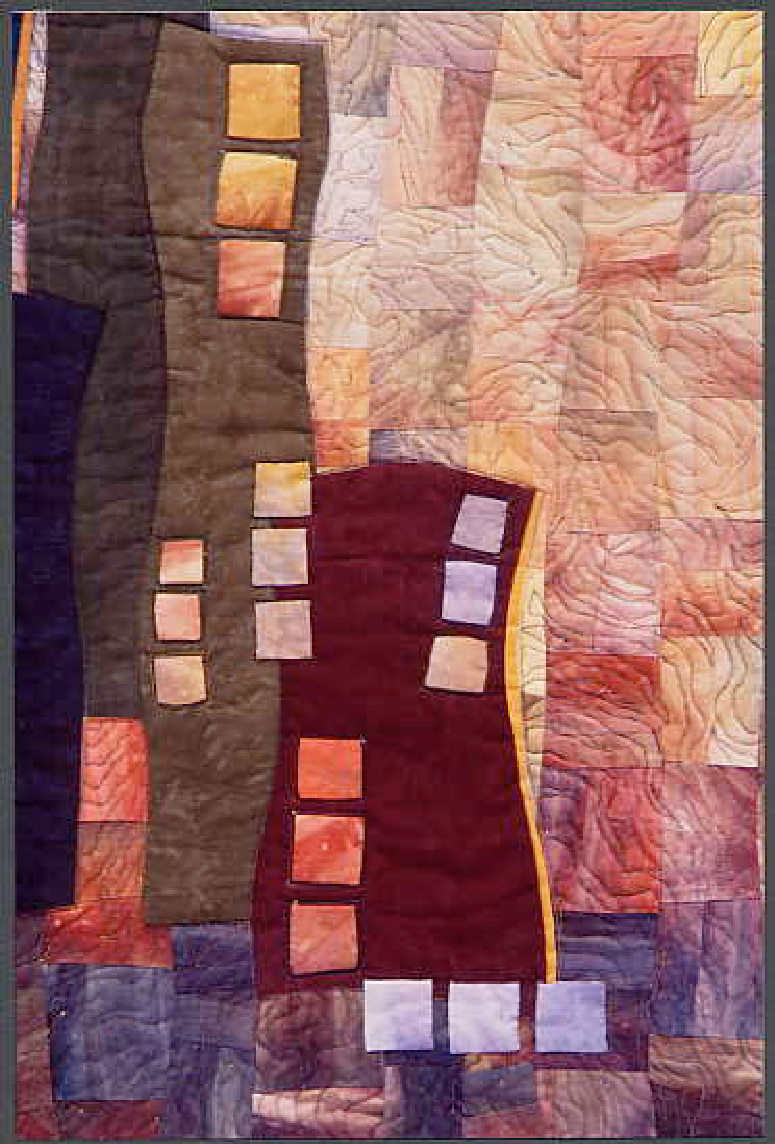
\epsfig{file=logo.pdf, height=2in}
\else
  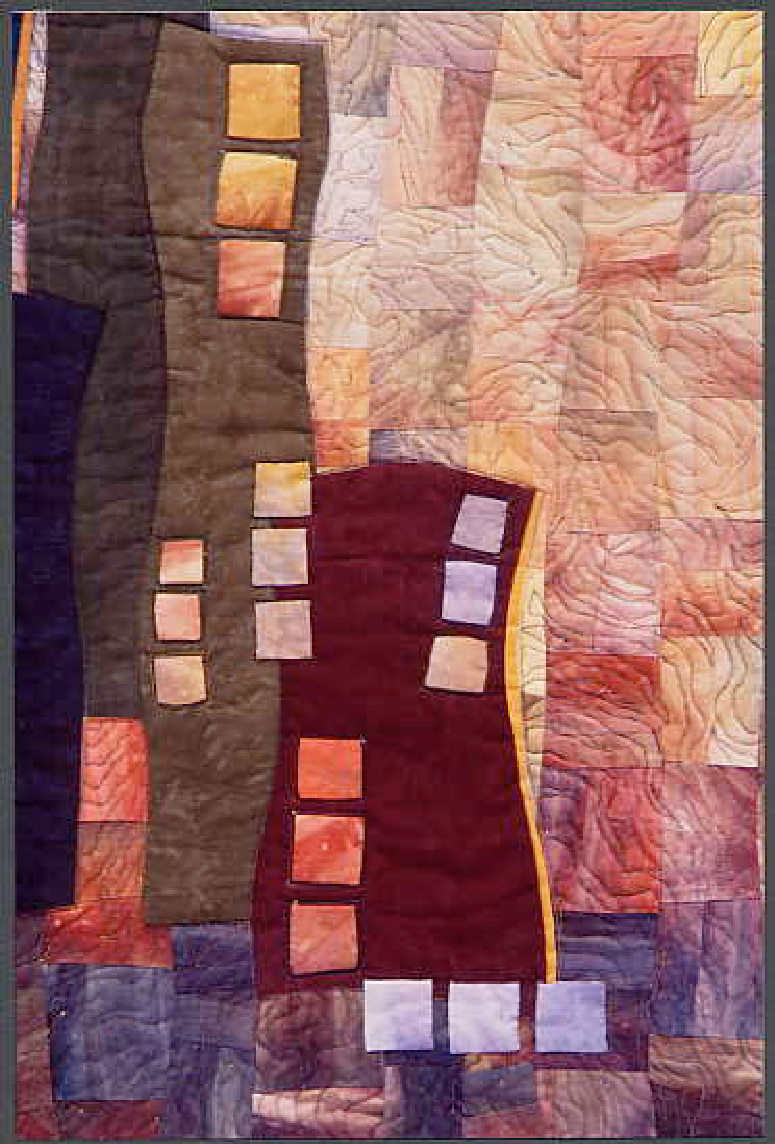
\includegraphics{logo.ps}
\fi
\end{center}


{\LARGE{}\DocumentTitle{}}

\vspace*{0.5in}

\DocumentAuthor{}

{\Large Last revised: \RevDate{}} \\

\vspace*{0.5in}
\centerline{
  \CopyrightMsg
}

\end{latexonly}%
%HEVEA \begin{center}
%HEVEA \begin{rawhtml} <IMG SRC="logo.jpg" height="200">\end{rawhtml}
%HEVEA \vspace*{0.25in}
%HEVEA {\LARGE{}\DocumentTitle{}}
%HEVEA \vspace*{0.25in}
%HEVEA \DocumentAuthor{}
%HEVEA \vspace*{0.25in}
%HEVEA Last revised: \RevDate{} \\
%HEVEA \vspace*{0.25in}
%HEVEA \CopyrightMsg{} \\
%HEVEA \end{center}

\end{titlepage}%


\cleardoublepage
\pagestyle{plain}
\pagenumbering{roman}

\setcounter{page}{1}
\begin{latexonly}
\tableofcontents
\end{latexonly}
\chapter*{Preface}\cutname{preface.html}
\addcontentsline{toc}{chapter}{Preface}
\section*{Acknowledgments}
\addcontentsline{toc}{section}{Acknowledgements}
We would like to thank Bala Krishnamurthy, Andrew Hume, David Poole,
and Oliver Spatscheck
for informative discussions about particular forms of ad hoc data
and potentially useful tools for manipulating that data.  
We would like to thank Glenn Fowler and Phong Vo for their help in
using the AST and SFIO libraries.
We would like to thank Mary Fernandez, Ricardo Medel, and Yitzhak
Mandelbaum for their assistance in integrating PADS and Galax.
Xuan Zheng implemented the histogram library.




\cleardoublepage
\setcounter{page}{1}
\pagenumbering{arabic}


\section{Introduction}
\label{sec:intro}

{\em Data description languages} are a class of domain specific
languages for specifying {\em ad hoc data formats}, from billing 
records to TCP packets to scientific data sets to server logs.  Examples 
of such languages include 
\bro~\cite{paxson:bro}, \datascript{}~\cite{gpce02}, \demeter~\cite{lieberherr+:class-dictionaries},
\packettypes{}~\cite{sigcomm00}, \padsc{}~\cite{fisher+:pads}, 
\padsml{}~\cite{mandelbaum+:padsml}  and
\xsugar~\cite{xsugar2005}, among others.  All of these languages
generate parsers from data descriptions.  In addition, and unlike
conventional parsing tools such as Lex and Yacc, many also automatically
generate auxiliary tools ranging from printers to \xml{} converters to
visitor libraries to visualization and editor tools.

In previous work, we developed the {\em Data Description Calculus}
(\ddcold{}), a calculus of simple, orthogonal type constructors,
designed to capture the core features of many existing type-based data
description languages~\cite{fisher+:next700ddl,fisher+:ddcjournal}.
This calculus had a multi-part denotational semantics that interpreted
the type constructors as (1) parsers the transform external bit
strings into internal data representations and {\em parse descriptors}
(representations of parser errors), (2) types for the data
representations and parse descriptors, and (3) types for the parsers
as a whole.  We proved that this multi-part semantics was coherent in
the sense that the generated parsers always have the expected types
and generate representations that satisfy an important {\em
canonical forms} lemma.

The \ddcold{} has been very useful already, helping us debug and
improve several aspects of \padsc{}~\cite{fisher+:pads}, and serving
as a guide for the design of \padsml{}~\cite{mandelbaum+:padsml}.
However, this initial work on the \ddcold{} told only a fraction of the
semantic story concerning data description languages.  As mentioned
above, many of these languages not only provide parsers, but
also other tools.  Amongst the most common auxiliary tools
are printers, as reliable communication between programs, either through
the file system or over the Web, depends upon both input (parsing) 
and output (printing).

In this work, we begin to address the limitations of
\ddcold{} by specifying a printing semantics for the
various features of the calculus.  We also
prove a collection of theorems for the new semantics that serve as
duals to our theorems concerning parsing.  This new printing semantics
has many of the same practical benefits as our older parsing 
semantics: We can
use it as a check against the correctness of our printer
implementations and as a guide for the
implementation of future data description languages.  


% First, we extend \ddcold{} with
% abstractions over types, which provides a basis for specifying the
% semantics of \padsml{}. In the process, we also improve upon the
% \ddcold{} theory by making a couple of subtle changes. For example, we
% are able to eliminate the complicated ``contractiveness'' constraint
% from our earlier work. Second, .

% The main practical benefit of the calculus has been as a guide for our
% implementation. Before working through the formal semantics, we
% struggled to disentangle the invariants related to polymorphism. After
% we had defined the calculus, we were able to implement type
% abstractions as \ocaml{} functors in approximately a week.  Our new
% printing semantics was also very important for helping us define and
% check the correctness of our printer implementation.  We hope the
% calculus will serve as a guide for implementations of \pads{} in
% other host languages.  

% In summary, this work makes the following key contributions:
% \begin{itemize}
% \item We simultaneously specify both a parsing and a printing semantics
%   for the \ddc{}, a calculus of polymorphic, dependent types.
% \item We prove that \ddc{} parsers and printers are type safe
%   and well-behaved as defined by a canonical forms theorem.
% \end{itemize}

In this extended abstract, we give an brief overview of the calculus,
it's dual semantics and their properties.  A companion technical
report contains a complete formal
specification~\cite{fisher+:popl-sub-long}.  In comparison to our
previous work on the \ddcold{} at POPL 06~\cite{mandelbaum+:padsml},
the calculus we present here has been streamlined in several subtle,
but useful ways.  It has also been improved through the addition of
polymorphic types.  We call this new polymorphic variant
\ddc{}.  These improvements and extensions, together with
proofs, appear in Mandelbaum's thesis~\cite{mandelbaum:thesis} and in
a recently submitted journal article~\cite{fisher+:ddcjournal}.
This abstract reviews the \ddc{} and extends all the previous 
work with a printing semantics and appropriate theorems.
To be more specific,
sections~\ref{sec:ddc-syntax} through \ref{sec:ddc-sem} present the
extended \ddc{} calculus, focusing on the semantics of polymorphic
types for parsing and the key elements of the printing semantics.
Then, \secref{sec:meta-theory} shows that both parsers and
printers in the \ddc{} are type correct and furthermore that parsers
produce pairs of parsed data and parse descriptors in {\em canonical
  form}, and that printers, given data in canonical form, print
successfully. We briefly discuss related work in \secref{sec:related}, and
conclude in \secref{sec:conc}.

%%% Local Variables: 
%%% mode: latex
%%% TeX-master: "paper"
%%% End: 

\chapter{Example}
\label{chap:example}
In this chapter, we use examples to give an overview of \pads{}.

\section{CLF: Common log format}
\label{sec:example:common-log-format}
The Common Log Format (CLF) \cite{clf} for web proxy/servers is used
to describe client request/server response pairs.  Such logs consist
of a sequence of entries, each of which contains information about a
single request/response.  In particular, each entry specifies the IP
address/hostname of the client, the owner of the TCP connection if
known, the authenticated user makeing the request if known, the time
of the request, the HTTP method used, the requested URL, the HTTP
version, a three-digit response code, and the number of bytes
returned. 

\begin{verbatim}
207.136.97.49 - - [15/Oct/1997:18:46:51 -0700] "GET /tk/p.txt HTTP/1.0" 200 30
include other record formats here.
\end{verbatim}

\section{\padsl{} description}
\label{sec:example:padsl-description}
Include top-down presentation of pads description

\section{Generated library}
\label{sec:example:generated-library}
Explain outputs of library.
%\begin{figure*}
\begin{code}
\kw{typedef} \kw{struct} \{
  Pbase\_m compoundLevel;   // Struct-level controls, eg., check Pwhere clause
  order\_header\_t\_m h;
  eventSeq\_t\_m events;
\} entry\_t\_m;
\mbox{}
\kw{typedef} \kw{struct} \{
  Pflags\_t pstate;         // Normal, Partial, or Panicking 
  Puint32 nerr;            // Number of detected errors.
  PerrCode\_t errCode;      // Error code of first detected error
  Ploc\_t loc;              // Location of first error
  order\_header\_t\_pd h;     // Nested header information
  eventSeq\_t\_pd events;    // Nested event sequence information
\} entry\_t\_pd;
\mbox{}
\kw{typedef} \kw{struct} \{
  order\_header\_t h;
  eventSeq\_t events;
\} entry\_t;
\end{code}

\begin{code}
/* Core parsing library */
Perror\_t entry\_t\_read (P\_t *pads,entry\_t\_m *m,entry\_t\_pd *pd,entry\_t *rep);
ssize\_t entry\_t\_write2io (P\_t *pads,Sfio\_t *io,entry\_t\_pd *pd,entry\_t *rep);
\end{code}

\begin{code}
/* Selected utility functions */
\kw{void} entry\_t\_m\_init (P\_t *pads,entry\_t\_m *mask,Pbase\_m baseMask);
\kw{int} entry\_t\_verify (entry\_t *rep);
\end{code}

\begin{code}
/* Selected accumulator functions */
Perror\_t entry\_t\_acc\_init (P\_t *pads,entry\_t\_acc *acc);
Perror\_t entry\_t\_acc\_add (P\_t *pads,entry\_t\_acc *acc,entry\_t\_pd *pd,entry\_t *rep);
Perror\_t entry\_t\_acc\_report (P\_t *pads,\kw{char} \kw{const} *prefix,\kw{char} \kw{const} *what,
                             \kw{int} nst,entry\_t\_acc *acc);
\end{code}

\begin{code}
/* Formatting */
ssize\_t entry\_t\_fmt2io (P\_t *pads,Sfio\_t *io,\kw{int} *requestedOut,
                        \kw{char} \kw{const} *delims,entry\_t\_m *m,entry\_t\_pd *pd,entry\_t *rep);
\end{code}

\begin{code}
/* Conversion to XML */
ssize\_t entry\_t\_write\_xml\_2io (P\_t *pads,Sfio\_t *io,entry\_t\_pd *pd,
                               entry\_t *rep,\kw{char} \kw{const} *tag,\kw{int} indent);
\end{code}

\begin{code}
/* Galax Data API */
PDCI\_node\_t *entry\_t\_node\_new (PDCI\_node\_t *parent,\kw{char} \kw{const} *name,\kw{void} *m,
                               \kw{void} *pd,\kw{void} *rep,\kw{char} \kw{const} *kind,\kw{char} \kw{const} *whatfn);
PDCI\_node\_t *entry\_t\_node\_kthChild (PDCI\_node\_t *self,PDCI\_childIndex\_t idx);
\end{code}

\label{figure:library}
\caption{Selected portions of generated library for \texttt{entry\_t}
  declaration from Dibbler data description.}
\end{figure*}
\chapter{Common features}
In this chapter, we describe \PADSL{} features shared by all types. 
Subsequent chapters describe features particular to various \PADSL{}
types. 

\section{\pads{} types}
\label{sec:common-overall}
Each \padsl{} type specifies the external representation of a
particular kind of data.  \padsl{} base types describe the
representations of atomic pieces of data, while structured types
specify how compound representations are built from more basic ones. 
\padsl{} provides a large and extensible collection of base types
and a family of type constructors for building structured types: 
\pstruct{}s for record-like sequences, 
\punion{}s for alternatives, 
\parray{}s for sequences, 
\penum{}s for fixed collections of strings, and
\ptypedef{}s for refinements of existing types.

Syntactically, a \padsl{} type (\nont{p\_ty}) must have the following form:

\vskip 1ex
\begin{tabular}{rcll}
\nont{p\_ty} & \is{} & \nont{base\_ty} & (* \chapref{chap:base-types} *) \\[1ex]
& \alt{} & \nont{struct\_ty}           & (* \chapref{chap:structs} *)\\[1ex]
& \alt{} & \nont{union\_ty}            & (* \chapref{chap:unions} *)\\[1ex]
& \alt{} & \nont{array\_ty}            & (* \chapref{chap:arrays} *)\\[1ex]
& \alt{} & \nont{enum\_ty}             & (* \chapref{chap:enums} *)\\[1ex]
& \alt{} & \nont{typedef\_ty}          & (* \chapref{chap:typedefs} *)\\[1ex]
\end{tabular}

\noindent
The grammar for each of the above non-terminals is given in the
associated chapter.

\section{Comments}
\label{sec:common-comments}
In addition to \C{} and \Cplusplus{} style comments of the form 
\cd{/* ... */} and \cd{//...}, which may appear anywhere in a \pads{}
description, \padsl{} also supports \nont{p\_comment}s, which may
appear only in particular locations in the grammar.  Syntactically,

\vskip 1ex
\begin{tabular}{rcll}
\nont{p\_comment} & \is{} & \cd{/-} text  \\[1ex]
\end{tabular}

\noindent
These comments are reflected to the generated \texttt{.h} file as documentation.



\section{Predicates}
\label{sec:common-predicates}
 written in C. integer type
 assumed to be side-effect free
 \term{predicate}

\section{Literals}
\label{sec:common-literals}

\begin{tabular}{l}
\term{char\_lit} \\[1ex]
\term{str\_lit} \\[1ex]
\end{tabular}

\PADSL{} supports C-style character and string literals such as {\tt '}\cd{a}{\tt '} and
\cd{"foo"}.  These literals may use all of C character escapes such as
\begin{verbatim}\" and \'\end{verbatim}
.

Character and string literals are used to read external characters
without putting any corresponding data in the resulting in-memory representation.
\Ie, they 'skip over' some expected character(s).
They are typically used in \Pstruct{}s; see \secref{sec:sec:structs-literal-fields}.

\section{Character Sets}
\label{sec:common-character-sets}

The library discipline contains a field \cd{def_charset} that
indicates the expected character set of the external representation of
character and string literals, as well as the external representation of all character and string
base types that do not explicitly name a character set.  Supported
character sets include ASCII (\cd{PDC_charset_ASCII}) and EBCDIC
(\cd{PDC_charset_EBCDIC}), where ASCII is the default character set.
\secref{sec:library-customization-character-encodings} describes how
to set \cd{def_charset}.

\section{White Space}
\label{sec:common-features-white-space}
Is there anything we need to say here?

\section{Parameterization}
\label{sec:common-parameterization}
To reduce the number of necessary type declarations and to permit the
format of later portions of the data to depend upon earlier portions, 
\PADSL{} types can be parameterized by values.  A common example of
the latter use is a data source which first specifies the length of a
sequence and then gives the sequence itself.  The length is read,
stored in the in-memory representation, and then passed to the type
that describes the sequence to specify the termination condition for
the sequence. Syntactically, 
\vskip 1ex
\begin{tabular}{rcl}
\nont{p\_actuals} & \is{} & \nont{expression} \alt{} \nont{expression}, \nont{p\_actuals} \\[1ex]
\nont{p\_actual\_list} & \is{} & (: \nont{p\_actuals} :)\\[2ex]
\end{tabular}

\noindent
where \nont{expression} is any \C{} expression. Formal parameter lists
\nont{formals} are the same as in \C{}. 

\subsection{Example}
The following \padsl{} fragment illustrates both declaring and passing
parameters to \pads{} types.
\begin{code}
\input{code/struct.parameters}
\end{code}

\section{\Precord{} modifier}

\section{\Pfile{} modifier}

\section{Error model}
\label{sec:common-error-model}
 panic versus non-panic errors



\section{In-memory representations}
\label{sec:common-rep}
Each \PADS{} type \cd{foo} has an associated in-memory representation
type of the same name.  The structure of this representation depends
upon the particular \PADS{} type.  
In general, these representations fall into two broad categories:
\textit{static} representations, whose size can be computed at
library-generation time, and \textit{dynamic} representations, whose size 
depends on the data being parsed. 
Details appear in 
\secref{sec:base-types-rep}, \secref{sec:structs-rep},
\secref{sec:unions-rep}, \secref{sec:arrays-rep}, 
\secref{sec:enums-rep}, and \secref{sec:typedefs-rep}.

\section{Masks}
\label{sec:common-masks}
Each \PADS{} type \cd{foo} has an associated mask type, \csmSuf{foo}.
Masks allow the library user to customize operations on portions of
the associated data.  The structure of the mask for a given \PADS{}
type mirrors the structure of the representation type.  Details about
the structure for various types
appear in \secref{sec:base-types-masks}, \secref{sec:structs-masks},
\secref{sec:unions-masks}, \secref{sec:arrays-masks}, 
\secref{sec:enums-masks}, and \secref{sec:typedefs-masks}.


\section{Parse descriptors}
\label{sec:common-parse-descriptor}
Each \PADS{} type \cd{foo} has an associated parse descriptor type, 
\pdSuf{foo}, coded as a \C{} struct with at least the following four
fields:
\vskip 1ex
\begin{tabular}{lp{4in}}
 \cd{PDC\_uint32 pstate} & Flags that describe the state after parsing the
                           associated value.\\[1ex]
 \cd{PDC\_errCode\_t errCode} & A code indicating the nature of the 
                               first detected error.\\[1ex]
 \cd{PDC\_loc\_t loc}  & The location in the data source of the first 
                         error.\\[1ex]
 \cd{PDC\_uint32 nerr} & The number of errors detected during parsing
                        of the associated value.\\[1ex]
\end{tabular}

\noindent
Field \cd{pstate} contains the following flags:
\vskip 1ex
\begin{tabular}{lp{3.5in}}
 \cd{PDC\_Panic} & Set if the parser was in panic mode during the
                  parsing of the associated data.\\[1ex]
\end{tabular}

\noindent
The \pads{} library provides a collection of functions (macros
actually) for manipulating the parse state field:
\vskip 1ex
\begin{code}
void PDC_PS_init(void *pd);         
void PDC_PS_setPanic(void *pd);     
void PDC_PS_unsetPanic(void *pd);   
int  PDC_PS_isPanic(void *pd);      
\end{code}

\cd{errCode}: \appref{app:error-codes} contains a list of all error codes and
describes their meanings.

\cd{loc} : describe the structure of this data.

Details about how parse descriptors are customized for various \PADS{}
types appear in
\secref{sec:base-type-parse-descriptors}, \secref{sec:structs-parse-descriptors},
\secref{sec:unions-parse-descriptors}, \secref{sec:arrays-parse-descriptors}, 
\secref{sec:enums-parse-descriptors} and \secref{sec:typedefs-parse-descriptors}.

\section{Regular Expressions}
\label{sec:regular-expressions}

XXX TODO.  

Need to describe semantics currently supported.

Need to describe compiled (type \PDCregexpt{}) vs. strings.

Mention uses:  library discipline, read functions.


\section{Operations}
\label{common-operations}
For each \pads{} type, the generated library contains a collection of
functions for manipulating the associated data.  For structured types,
the \pads{} compiler generates these functions;  for base types, the
\pads{} library provides them.  This section describes the common
features of such functions.  Type-specific information may be found in
the appropriate chapter.

All operations take a pointer to an
initialized \pads{} handle as their first parameter.  Information
about how to manage \pads{} library handles appears in
\chapref{chap:using-library}. 

Many of the operations that can fail return a value of type
\cd{PDC\_error\_t} to indicate success or failure.  This type has two
values: \cd{PDC\_OK} and \cd{PDC\_ERROR}. 


\subsection{Initialization and cleanup functions}
For each type \cd{foo}, the generated library contains
initialization and cleanup functions for the associated representation
\cd{foo} and parse descriptor \pdSuf{foo} types.  Each initialization
function take a pointer to allocated space and initializes the space
appropriately.  Each cleanup function takes a pointer to allocated and
initialized space and deallocates any memory allocated by \pads{} functions.
It does not deallocate the space pointed to by the parameter.  
\begin{code}
PDC_error_t foo_init (PDC_t *pdc, foo *rep);

PDC_error_t foo_cleanup (PDC_t *pdc, foo *rep);

PDC_error_t foo_pd_init (PDC_t *pdc, foo_pd *pd);

PDC_error_t foo_pd_cleanup (PDC_t *pdc, foo_pd *pd);
\end{code}
Because all masks have statically-known size, the library does not
contain initialization and cleanup functions for masks.  
\begin{code}
void foo_m_init (PDC_t *pdc, foo_m *mask, PDC_base_m baseMask);
\end{code}
Instead, it
contains a function for setting all nested base masks 
to a specified value.  The function takes two parameters (in
addition to the \pads{} handle): a pointer to allocated space for the
mask and a base mask value.  Because mask initialization
functions cannot fail, the return type is \cd{void} instead of
\cd{PDC_error_t}. 

\subsection{Utilty functions}
Each type \cd{foo} comes equipped with copy functions for both the
in-memory representation and the parse descriptor.  Both the source
and destination pointers are assumed to point to allocated space.  In
addition, the src pointers are assumed to point to initialized space.
\begin{code}
PDC_error_t foo_copy (PDC_t *pdc, foo *rep_dst, foo *rep_src);

PDC_error_t foo_pd_copy (PDC_t *pdc, foo_pd *pd_dst, foo_pd *pd_src);
\end{code}

\subsection{Read function}
The read function for a \pads{} type \cd{foo} takes as an input parameter a
pointer to a mask \cd{m} and returns as output parameters a pointer to
a parse descriptor \cd{pd} and a pointer to an in-memory
reprsentation \cd{rep}.  If any errors occurred during the parsing, the return
value for the function is \cd{PDC_ERROR}.  Otherwise, the function
will return \cd{PDC_OK}.  

\begin{code}
PDC_error_t foo_read (PDC_t *pdc, foo_m *m, foo_pd *pd, foo *rep);
\end{code}

The mask argument allows the library user to specify independently
which constraints the parser should check and which portions of the
in-memory representation it should fill in.  Conceptually, there are
three different ``knobs'' associated with each atomic element of a
\pads{} type:

\vskip 1ex
\begin{tabular}{ll}
\cd{PDC_SynCheck} & Check syntactic constraints\\
\cd{PDC_SymCheck} & Check semantic constraints\\
\cd{PDC_Set}      & Set the in-memory reprsentation\\[1ex]
\end{tabular}

\noindent
At the base-type level, the mask consists of one or more of the
above flags.
For structured types, the mask consists of a combination of base masks
and the masks associated with nested types, the exact combination of
which depends upon the kind of structured type.  Note that for a
structured type \cd{foo}, the mask initialization function
\cd{foo_m_init} can be used to initialize all nested masks to the
supplied value.

Details about the read functions for particular types may be found in
the appropriate chapters.

For convenience, the \pads{} library provides the following abbreviations:

\vskip 1ex
\begin{tabular}{ll}
\cd{\#define PDC\_CheckAndSet} & \cd{PDC\_Set|PDC\_SynCheck|PDC\_SemCheck}\\
\cd{\#define PDC\_BothCheck}   & \cd{PDC\_SynCheck|PDC\_SemCheck} \\
\cd{\#define PDC\_Ignore}      & no flags set\\[1ex]
\end{tabular}

\noindent
The library also provides the following macros for testing or
modifying base read-function flags:

\vskip 1ex
{\small
\begin{tabular}{ll}
\cd{\#define PDC\_Test\_Set(m)}            & \cd{(m \& PDC\_Set)} \\
\cd{\#define PDC\_Test\_SynCheck(m)}       & \cd{(m \& PDC\_SynCheck)}\\
\cd{\#define PDC\_Test\_SemCheck(m)}       & \cd{(m \& PDC\_SemCheck)}\\
\\
\cd{\#define PDC\_Test\_NotSet(m)}         & \cd{(!PDC\_Test\_Set(m))}\\
\cd{\#define PDC\_Test\_NotSynCheck(m)}    & \cd{(!PDC\_Test\_SynCheck(m))}\\
\cd{\#define PDC\_Test\_NotSemCheck(m)}    & \cd{(!PDC\_Test\_SemCheck(m))}\\
\\
\cd{\#define PDC\_Test\_CheckAndSet(m)}    & \cd{((m \& PDC\_CheckAndSet) == PDC\_CheckAndSet)}\\
\cd{\#define PDC\_Test\_BothCheck(m)}      & \cd{((m \& PDC\_CheckAndSet) == PDC\_BothCheck)}\\
\cd{\#define PDC\_Test\_Ignore(m)}         & \cd{((m \& PDC\_CheckAndSet) == PDC\_Ignore)}\\
\\
\cd{\#define PDC\_Test\_NotCheckAndSet(m)} & \cd{((m \& PDC\_CheckAndSet) != PDC\_CheckAndSet)}\\
\cd{\#define PDC\_Test\_NotBothCheck(m)}   & \cd{((m \& PDC\_CheckAndSet) != PDC\_BothCheck)}\\
\cd{\#define PDC\_Test\_NotIgnore(m)}      & \cd{((m \& PDC\_CheckAndSet) != PDC\_Ignore)}\\
\\
\cd{\#define PDC\_Do\_Set(m)}              & \cd{(m |= PDC\_Set)}\\
\cd{\#define PDC\_Do\_SynCheck(m)}         & \cd{(m |= PDC\_SynCheck)}\\
\cd{\#define PDC\_Do\_SemCheck(m)}         & \cd{(m |= PDC\_SemCheck)}\\
\\
\cd{\#define PDC\_Dont\_Set(m)}            & \cd{(m \&= (~PDC\_Set))}\\
\cd{\#define PDC\_Dont\_SynCheck(m)}       & \cd{(m \&= (~PDC\_SynCheck))}\\
\cd{\#define PDC\_Dont\_SemCheck(m)}       & \cd{(m \&= (~PDC\_SemCheck))}\\[1ex]
\end{tabular}
}
\subsection{Write functions}
For each \pads{} type, the generated library provides 
two functions for writing out the in-memory representation of the type
in a format as close as possible to its original form.
\begin{code}
ssize\_t foo\_write2io (PDC\_t *pdc, Sfio\_t *io, foo\_pd *pd, foo *rep);

ssize\_t foo\_write2buf (PDC\_t *pdc, PDC\_byte *buf, size\_t buf\_len, 
                        int *buf\_full, foo\_pd *pd, foo *rep);
\end{code}
The first of these functions emits its output to an SFIO file;
the second to an in-memory buffer.  Information about SFIO may be
found from \url{www.research.att.com/sw/tools/sfio}.  For the buffer
version, the parameter \cd{buf} points to an allocated sequence of
bytes and \cd{buf\_len} indicates the size of the buffer.  Out
parameter \cd{buf\_full} is a boolean which is set if the requested
write would have overflowed the buffer. The return value
for both of the functions is the number of bytes written, with \cd{-1}
indicating an error occurred.  

Issues that may cause the written data to differ from the original
data include skipping white space
(\secref{sec:library-customization-white-space}) and omitting fields in
\Pstruct{}s (\secref{sec:structs-qualifiers}). 

Passing the \texttt{-wnone} flag to the \pads{} compiler suppresses
the generation of these functions for structured types.

We anticipate adding more write functions in the future.

\subsection{Additional functions}
In addition to the basic functionality described in the preceeding
sections, \pads{} provides more advanced features described in later
chapters. 

\begin{tabular}{lp{4in}}
Accumulators (\chapref{chap:accumulators})  & Provide structures and
functions for automatically summarizing data.\\
\end{tabular}


\chapter{Base Types Overview}
\label{chap:base-types}
\cutname{base.html}

\PADSL{} base types describe inidivual, small values: numbers, strings, dates, and so on.
This chapter provides an overview of some of the most important built-in \PADSL{} base types,
with a focus on how these types are used within \PADSL{} source files.
\appref{ap:base-types} gives detailed descriptions of each of the built-in base types,
including the full set of library API calls for each type.  (As discussed in
\chapref{chap:common-features}, each type has correspond read, write,
format, and accumulator functions.) 

In addition to the built-in types, it is possible to extend \PADSL{} with 
new base types; see \secref{sec:library-adding-new-base-types}.

\section{In-Memory Representation}
\label{sec:base-types-rep}

Each base type has an external and an in-memory representation. 
Related base types share the same in-memory representation.  For
example, while there are 18 different string base types, all of them
use \Pd{string} as their in-memory representation.

This section reviews the different in-memory representation types.

\subsection{{\tt Pchar}}

Type \Pd{char} is the in-memory representation of an external
character.  It is equivalent to the C type \cd{unsigned char}, or type
\Pd{uint8}: all are 8-bit unsigned values.  {\bf N.B.}: Regardless of the
external character that is read, the corresponding ASCII character is stored in 
the in-memory representation.

\subsection{{\tt Pstring}}

Type \Pd{string} is the in-memory representation for all forms of
external strings.  A \Pd{string} \cd{s} has two fields:
\begin{itemize}
\item \cd{s.len} : the length of the string.
\item \cd{s.str} : a pointer to a sequence of \cd{s.len} characters.
\end{itemize}
In addition, \Pd{string} has fields that are manipulated
by various string functions (some of which are described below).
Most programmers should only use \cd{s.len} and \cd{s.str}.

The library discipline has a field \cd{copy\_strings} which controls
copying behavior for string read calls.  If \cd{copy\_strings} is
non-zero, the string read functions always copy strings. Otherwise, a
copy is not made and the target \Pd{string} points to memory managed by
the current IO discipline.  \cd{copy\_strings} should only be set to
zero for record-based IO disciplines where strings from record K are
not used after \Pd{\_io\_next\_rec} has been called to move the IO cursor
to record K+1.  Note: \Pd{string\_preserve} can be used to force
a string that is using sharing to make a copy so that the string is
'preserved' (remains valid) across calls to \Pd{\_io\_next\_rec}.

When copying is used, the string copies are stored in an internal
resizable buffer, and \cd{s.str} points into this buffer. 
To ensure correct behavior, function \Pd{string\_init} should be called
prior to using a \Pd{string}, and function \Pd{string\_cleanup} should
be called when a given \Pd{string} is no longer in use.
Generated initialization and cleanup functions call these routines for
any \pads{} type containing a \Pd{string}.

The full set of string helper functions appears in \figref{fig:string-functions}.
\begin{figure}
\inputCode{code/strings}
\caption{Library functions for manipulating \texttt{Pstring}s.}
\label{fig:string-functions}
\end{figure}

The following list describes the behaviors of these functions.
\begin{description}
\item[\cd{Pstring\_init(pads, s)}] 
  Initialize \cd{s} to valid empty string (no dynamic memory allocated yet).
\item[\cd{Pstring\_cleanup(pads, s)}] 
  Free any dynamic memory allocated for \cd{s}.
\item[\cd{Pstring\_share(pads, targ, src)}] 
  Make \cd{targ} refer to the string in \cd{src}, sharing the space with the original owner.
\item[\cd{Pstring\_cstr\_share(pads, targ, src, len)}] 
  Make \cd{targ} refer to \cd{len} characters in C-string \cd{src}.
\item[\cd{Pstring\_copy(pads, targ, src)}]
  Copy the string in \cd{src} into \cd{targ}; sharing is not used.
\item[\cd{Pstring\_cstr\_copy(pads, targ, src, len)}] 
 Copy \cd{len} characters from C-string \cd{src} into \cd{targ}; sharing is not used.
\item[\cd{Pstring\_eq(str1, str2)}] 
 Returns \cd{1} if \cd{str1} and \cd{str2} are of equal length and
 \cd{str1} equals \cd{str2} (based on strncmp). Otherwise, returns \cd{0}.
\item[\cd{Pstring\_eq\_cstr(str, cstr)}]
 Returns \cd{1} if \cd{str1} and \cd{str2} are of equal length and
 \cd{str1} equals \cd{str2} (based on strncmp). Otherwise, returns \cd{0}.
\end{description}

Although not strictly necessary, both \Pd{string\_copy} and
\Pd{string\_cstr\_copy} null-terminate \cd{targ->str}.  Each copy
function returns \Pd{\_ERR} on bad arguments or on failure to allocate
space, otherwise it returns \Pd{\_OK}.

The various Pstring2NUMERIC functions convert a string to the
specified numeric type.  If the contents of the string cannot be
converted to the specified type, the minumum value for the numeric
type is returned for signed numeric types, or the maximum value is
returned for unsigned numeric types.

\subsection{Integer types}

There are eight in-memory representations for integers, four types for
signed values (\Pd{int8}, \Pd{int16}, \Pd{int32}, and \Pd{int64})
and four types for unsigned values (\Pd{uint8}, \Pd{uint16}, \Pd{uint32}, and \Pd{uint64}).
The number in these type names indicates the number of bits in the in-memory representation,
thus there are signed and unsigned integers that use 1, 2, 4, or 8 bytes of memory.
The endian-ness of these in-memory representation types is the same as the
endian-ness of the processor that the code is executing on. 
The external representation, which may be in another format, is always converted
to the primitive in-memory representation supported by the processor.

For programming convenience, the header file {\tt pads.h} includes definitions of the minimum
and maximum values for each signed type, and of the maximum value for
each unsigned type.  \figref{fig:limits} list these constants.
\begin{figure}
\inputCode{code/limits}
\caption{Minimum and maximum values for \pads{} integer types.}
\label{fig:limits}
\end{figure}


\subsection{Floating-point types}

\PADSL{} has only two in-memory floating point representations,
\Pd{float32} and \Pd{float64}, which correspond to ANSI C types \cd{float}
and \cd{double}, respectively.

\subsection{Fixed-point types}

A fixed-point number is a number with a fixed number of decimal digits
(digits after the 'dot').  For example, 123.456 is a fixed-point
number with three decimal digits.  External formats for such numbers
occur, e.g., in COBOL data.  We have chosen a very simple in-memory
representation for such numbers: a struct with a numerator (\cd{num})
that contains all of the digits and a denominator (\cd{denom}) that
contains some power of 10.  For example, 123.456 would be represented
with a numerator containing 123456 and a denominator containing 1000 ($10^3$).

The in-memory representation always has an unsigned denominator. We
provide signed and unsigned representations that use signed and
unsigned numerators, respectively.  One can choose the number of bits
used for both numerator and denominator in the same way as for the
integer types, thus there are four types for signed values
and four types for unsigned values:

\inputCode{code/fixedpoint}

There are two macros to help one use values of these in-memory types.
\Pd{\_FPOINT2FLOAT32(fp)} calculates \cd{fp.num/fp.denom} as a \Pd{float32},
while \Pd{\_FPOINT2FLOAT64(fp)} calculates \cd{fp.num/fp.denom} as a \Pd{float64}.

\section{Base Type Mask}
\label{sec:base-type-mask}
The mask for base types is just an integer type, treated as an array
of bits:

\begin{centercode}
 typedef Puint32 Pbase\_m;
\end{centercode}
%
\noindent
Masks for accessing individual bits of the base type masks are described in
sections describing operations that use mask. (\cf{}
\secref{sec:common-features-read-function}). 
More information about how base types handle masks is available in
\appref{ap:base-types}

\section{Base Type Parse Descriptor}
\label{sec:base-type-parse-descriptors}
Parse descriptors for base types contain only the fields described in 
\secref{sec:common-parse-descriptor}.
Specific error codes are discussed when the base type read functions
are described.


\section{Character Sets}

\PADSL{} currently supports two character sets for external data, ASCII and EBCDIC.
As discussed in \secref{sec:common-character-sets}, the library
discipline contains a field
\cd{def\_charset} that selects which character set to use when
one is not specified explicitly.  As a result, for each 'kind' of data
that has an external form made up of characters (characters, strings,
character-based dates, character-based integer and floating point
numbers, \etc{}), \PADSL{} has three types: a type that indicates the external
form is always ASCII, a type that indicates the external form is
always EBCDIC, and a type that indicates that the external form uses
the character set specified in \cd{def\_charset}.

In each section describing character-based types, we give a
three-column table indicating the type(s) that use ASCII, EBCDIC, or
DEFAULT character sets.  For example, the next section begins with a
table showing types \Pa{char} (ASCII), \Pe{char} (EBCDIC), \Pd{char}
(DEFAULT).

\section{Character Base Types}

\subsection{Fixed-width character-based encoding}

\aedBegin{}
\aedLine{char}
\aedEnd{}
\myvskip{1ex}

\noindent
For example,  writing

\inputCode{code/char-decl}
%
\noindent
in a \PADSL{} source file (within a Pstruct, for example) indicates
that a single ASCII character is expected.  Writing a constraint
such as 

\inputCode{code/char-constraint-decl}
%
\noindent
indicates that an EBCDIC capital letter A or B is expected.
{\bf NB:}\/ Note that the constraint expression is applied to the
{\em in-memory\/} representation of c, which is an ASCII value,
thus the C character constants (ASCII constants)
are used to specify letters A and B.

\subsection{Special character counting base types}

\aedBegin{}
\aedLine{countX}
\aedLine{countXtoY}
\aedEnd{}

Unlike all other base types, these counting base types
never advance the IO cursor.  You can think of these types as
``peeking ahead'' to see how many occurrences of a given character
appear forward of the current IO cursor position.

The PcountX types count the number of occurences of character X
between the current IO cursor position and the fist EOR (end of
record) or EOF (end of file).  They take three parameters, \cd{x},
\cd{eor_required}, and \cd{count_max}.  \cd{x} is the character to count.  If
\cd{eor_required} is non-zero, then encountering EOF before EOR produces
an error.  If \cd{count_max} is non-zero, EOR/EOF must be encountered
before scanning \cd{count_max} characters, otherwise an error is returned.
For example,

\inputCode{code/countX}
%
\noindent
will count the number of ASCII equals-sign characters between
the IO cursor and the next EOR or EOF, with no limit on
the maximum scan distance.

\section{String Base Types (including dates and times)}

The large number of string base types arises from the fact that there
are many different ways to indicate the extent of a string.  The
entire input (up to end-of-file or end-of-record) is a sequence of
bytes that can be included in a string, so when specifying a string
type in a \padsl{} description, we need to indicate how much of that
input we would like included in the string.

\subsection{Pstring\_FW}

\aedBegin{}
\aedLine{string\_FW}
\aedEnd{}

One of the simplest ways to specify the extent of a string is to give the
exact number of characters, or width, that will be included in the string.
For example,
\inputCode{code/stringFW}
%
\noindent
Specifies a string with width 10.  In this case the default character set
will determine whether ASCII or EBCDIC characters are expected in the
input stream.  Regardless of the input character set, the resulting in-memory 
Pstring contains ASCII characters. 

An error occurs if the specified width is not available.  See \appref{ap:base-types}
for details.

\subsection{Pstring}

\aedBegin{}
\aedLine{string}
\aedEnd{}

For the Pstring type one specifies a 'stop character' that is
expected immediately {\em following\/} the string.  The extent of the
string is all characters from the IO cursor up
to but not including the first occurrence of the stop char.
For example,

\inputCode{code/string-stop}
%
\noindent
Indicates that a series of EBCDIC characters is expected, followed by
an EBCDIC vertical bar.  Note that the stop char is always specified
in ASCII (in this case usng a C character constant).  When the
character set that is being read from the input is EBCDIC, the read
function looks for the EBCDIC character that is equivalenet to the
specified ASCII character.

\subsection{Pstring\_ME}

\aedBegin{}
\aedLine{string\_ME}
\aedEnd{}

For type \cd{Pstring\_ME}, a regular expression called the {\em matching
expression\/} is given, and the extent of the string is the longest
sequence of characters starting at the current IO position which match
this expression.  Note that when you specify a regular expression as
a \C{} string, you must use two backslashes to indicate a single
backslash character (otherwise C will think you are applying the
special backslash operator to the following character). 
In a language such as Perl, which does not have this requirement,
you might write

\inputCode{code/reg-exp}
%
\noindent
to create a regular expression which will match a
sequence of zero or more non-space characters.  To use the
same regular expression in a PADSL description
with the \cd{Pa\_string\_ME} type, you would write:

\inputCode{code/string-match}
%
\noindent
This will match a sequence of zero or more non-space characters and assign
it to \cd{my\_string}.  Note that if a space occurs immediately, a match
still occurs, since we specified that zero characters was OK;
\cd{my\_string} would be a string of length zero.  The extent is bound be
end-of-record/end-of-file, so if there are no spaces before an
end-of-record, \cd{my\_string} will end up containing all characters
remaining in the record.

As a concrete example, if the input at the current IO cursor is {\tt hello
world} when the above string declaration is used to read from the
input, \cd{my\_string} will end up containing {\tt hello}.  Note that the
space that follows {\tt hello} is {\em not} included, since it does not
part of the match.

\subsection{Pstring\_SE}

\aedBegin{}
\aedLine{string\_SE}
\aedEnd{}

For type \cd{Pstring\_SE}, a regular expression called the {\em stop
expression\/} is given, and the extent of the string is the longest
sequence of characters starting at the current IO position such that
the characters immediately following successfully match the stop
expression.  None of the characters matching the stop expression
are included in the result.
For example,

\inputCode{code/string-stope}
%
\noindent
The stop expression will match {\em either\/} a space character (due to the backslash-s) {\em or\/}
end-of-record/end-of-file (due to the special dollar-sign character).  As a result,
\cd{my\_string} will end up containing all non-space characters up to (but not including) the 
first space characer that is found, or up to the end of the current record if no space
character is found.  

You may have noticed that the \cd{Pa\_string\_ME} and
\cd{Pa\_string\_SE} examples actually specify exactly the same extent.  
Because of the power of regular expressions, it is often the case that you can
choose to use either type.  You should use whichever type results in a
clearer description of what is expected in the input.  (In this case,
the\cd{Pa\_string\_ME} form is simpler and therefore clearer.)

\subsection{Timestamp\_explicit}

\begin{small}
\aedBegin{}
\aedLine{timestamp\_explicit\_FW}
\aedLine{timestamp\_explicit}
\aedLine{timestamp\_explicit\_ME}
\aedLine{timestamp\_explicit\_SE}
\aedEnd{}
\end{small}

\noindent
A timestamp is a combination of a calendar date and a time of day.
The corresponding in-memory representation is a \cd{Puint32} which
represents the number of seconds since {\tt 00:00:00 1-Jan-1970 UTC},
also knows as ``seconds since the epoch.''
Thus, the time {\tt 00:00:20 1-Jan-1970 UTC} would be represented
internally as the number 1200, since it occurs 1200 seconds
(20 minutes) past the epoch.

If the input is \texttt{``midnight Jan 1 1970''} and the time zone is \literal{UTC}, then
this produces a value of 0 since this is actually the epoch.  If the
time zone is \literal{EST}, then this produces 5 * 60 * 60 since midnight in the
\literal{EST} timezone occurred 5 hours after the start of the epoch.

If  the input explicitly has a time zone, as in \texttt{``midnight Jan 1 1970
UTC''} then the time zone in the input is used, so this would produce 0,
regardless of the time zone specified for the type.  Of course, not
all timestamp input formats allow you to explicitly give the time
zone!


The input values are ASCII or EBCDIC strings.  Each
\cd{Ptimestamp\_explicit} type takes as first argument the same form of
specifying the string's extent as the corresponding \cd{Pstring} type, and
takes as second argument a timestamp format string which describes
what the input string should contain.

Timestamp formats consists of literal characters that are are simply
expected to be present in the input and special combinations of a
percent-sign and a character used to indicate expected parts of the
timestamp.  For example, the input format
\literal{\cd{"\%Y-\%m-\%d+\%H:\%M"}} 
indicates that a format that starts with a 
four digit year, then a dash, then a two digit month, then a dash,
then a two-digit day, then a plus sign, then a two digit hour, then a
colon, then a two digit minutes.  (To specify that a literal percent
sign must appear in the input, use two percent signs in a row.)  A
full description of supported formats appears on the webpage:
\ifthenelse{\boolean{hevea}}{
\myurl{www.research.att.com/\~gsf/man/man3/tm.html}}{
\myurl{www.research.att.com/~gsf/man/man3/tm.html}}


Each of the \cd{Ptimestamp\_explicit} types corresponds to one of the \cd{Pstring}
types that has already been described, where each takes one additional argument
to specify the input format.  For example,

\inputCode{code/timestamp-explicit}
%
\noindent
Reads an ASCII string, up to but not including a vertical bar, and
converts that string into a \cd{Puint32} timestamp.  The conversion will be
successful only if the string has the specified format.

Some timestamp formats include explicit time zone information,such as
the one above.  \pads{} provides the function \cd{P\_cstr2timezone} to convert a
string representation of a time zone into an value of type
\cd{Tm\_zone\_t *}.  This function is described in \chapref{chap:library-use}.

For the rest,the input time zone is taken
from the \pads{} discipline field \cd{ disc->in\_time\_zone}, as
described in \secref{sec:library-customization-input-time-zone}.

\subsection{Timestamp}

\aedBegin{}
\aedLine{timestamp\_FW}
\aedLine{timestamp}
\aedLine{timestamp\_ME}
\aedLine{timestamp\_SE}
\aedEnd{}

The timestamp types are the same as the \cd{timestamp\_explicit} types,
except no timestamp format is given.  Instead, the \pads{}
discipline field \cd{disc->in\_formats.timestamp} is used
for all \cd{Ptimestamp} types.

\subsection{Date\_explicit}

\aedBegin{}
\aedLine{date\_explicit\_FW}
\aedLine{date\_explicit}
\aedLine{date\_explicit\_ME}
\aedLine{date\_explicit\_SE}
\aedEnd{}

Dates are calendar days (no time of day).  Like timestamps, we
represent a date as a \cd{Puint32} recording ``seconds since the epoch.''

The \cd{Pdate\_explicit} types take a second argument, a date format,
which accepts the same special characters as the \cd{Ptimestamp\_explcit} types.
So, technically there is nothing to stop you from using the date types
to input time of day fields.  However, we encourage you to use the
\cd{Ptimestamp} types when both a calendar day and a time of day are to be
input, and to use the \cd{Pdate} types when just the calendar day is to be
input.

\subsection{Date}

\aedBegin{}
\aedLine{date\_FW}
\aedLine{date}
\aedLine{date\_ME}
\aedLine{date\_SE}
\aedEnd{}

The date types are the same as the \cd{date\_explicit} types,
except no date format is given.  Instead, the \pads{}
discipline field \cd{disc->in\_formats.date} is used
for all \cd{Pdate} types.

\subsection{Time\_explicit}

\aedBegin{}
\aedLine{time\_explicit\_FW}
\aedLine{time\_explicit}
\aedLine{time\_explicit\_ME}
\aedLine{time\_explicit\_SE}
\aedEnd{}

Times give the time of day, with no calendar date.  They are
represented as a \cd{Puint32} recording seconds since midnight.  For
examle, the time 1am is represented as 3600 (i.e., 3600 seconds, or 60
minutes, after midnight).

The \cd{Ptime\_explicit} types take a second argument, a time format, which
accepts the same special characters as the timestamp and date types.
However, we encourage you to use the \cd{Ptimes} types when just a time of
day is expected.

\subsection{Time}

\aedBegin{}
\aedLine{time\_FW}
\aedLine{time}
\aedLine{time\_ME}
\aedLine{time\_SE}
\aedEnd{}

The time types are the same as the \cd{time\_explicit} types,
except no time format is given.  Instead, the \pads{}
discipline field \cd{disc->in\_formats.time} is used
for all \cd{Ptime} types.

\subsection{IP}

\aedBegin{}
\aedLine{ip\_FW}
\aedLine{ip}
\aedLine{ip\_ME}
\aedLine{ip\_SE}
\aedEnd{}

The \cd{Pip} type reads an IP address string from the input that is in
numeric dotted form (as in {\tt 10.1.0.17}) using ASCII or EBCDIC
digits and periods (dots).  The string consists of up to four
parts with values between 0 and 255, separated by periods,
with an optional trailing period.  When there are
fewer than four parts, the missing parts are treated as implicitly
zero, and are inserted as shown in the following diagram,
which shows the eight legal input forms and the equivalent expanded form.

{\tt
\begin{center}
\begin{tabular}{lcl}
  <part1>                          & ~~$\longrightarrow{}$~~ & <part1>.0.0.0\\
  <part1>.                         & ~~$\longrightarrow{}$~~ & <part1>.0.0.0.\\
  <part1>.<part4>                  & ~~$\longrightarrow{}$~~ & <part1>.0.0.<part4>\\
  <part1>.<part4>.                 & ~~$\longrightarrow{}$~~ & <part1>.0.0.<part4>.\\
  <part1>.<part2>.<part4>          & ~~$\longrightarrow{}$~~ & <part1>.<part2>.0.<part4>\\
  <part1>.<part2>.<part4>.         & ~~$\longrightarrow{}$~~ & <part1>.<part2>.0.<part4>.\\
  <part1>.<part2>.<part3>.<part4>  & ~~$\longrightarrow{}$~~ & same\\
  <part1>.<part2>.<part3>.<part4>. & ~~$\longrightarrow{}$~~ & same\\
\end{tabular}
\end{center}}

Each $<$part$>$ is made up of 1 to 3 digits which specify a number
in the range [0, 255].

The result is a single \cd{Puint32} value with each part encoded in one
of the four bytes.  part1 is stored in the high-order byte, part4
in the low-order byte.  You can obtain each part using the macro

\begin{centercode}
  P\_IP\_PART(addr, part)
\end{centercode}
where \cd{part} must be an integer between 1 and 4.

The digits and the "." char are read as EBCDIC chars if the EBCDIC
form is used or if the default form is used and
\cd{pads->disc->def\_charset} is \cd{Pcharset\_EBCDIC}.  Otherwise the data is
read as ASCII chars.

\section{Integer Base Types}

\subsection{Fixed-width character-based encoding}

\aedBegin{}
\aedLine{int8\_FW}
\aedLine{int16\_FW}
\aedLine{int32\_FW}
\aedLine{int64\_FW}
\aedLine{uint8\_FW}
\aedLine{uint16\_FW}
\aedLine{uint32\_FW}
\aedLine{uint64\_FW}
\aedEnd{}

The above types are used when the input representation for an integer
is a fixed number of ASCII or EBCDIC characters.  The \cd{int} types are
signed types, while the \cd{uint} types are unsigned.  The number in the
type name specifies how many bits are used in the in-memory
represenation, thus a \cd{Puint32} is a 32-bit (4 byte) representation of
an unsigned integer.

The characters in the input can have an optional plus or minus sign for
signed types, or an optional plus signed for unsigned types, followed
by a set of one or more digits.   In addition, leading or
trailing whitespace can occur, but only if the \pads{} discipline field
\cd{disc->flags} has the \cd{WSPACE\_OK} flag set.
The data is read as EBCDIC chars if an EBCDIC
form (such as \cd{Pe\_int8}) is used, or if the default form (\cd{Pint8}) is used and
\cd{pads->disc->def\_charset} is \cd{Pcharset\_EBCDIC}.  Otherwise, the data is
read as ASCII chars.

\subsection{Variable-width character-based encoding}

\aedBegin{}
\aedLine{int8}
\aedLine{int16}
\aedLine{int32}
\aedLine{int64}
\aedLine{uint8}
\aedLine{uint16}
\aedLine{uint32}
\aedLine{uint64}
\aedEnd{}

The expected input for these types is an optional sign character
followed by a sequence of digits.  The number of characters that make
the input is variable: after the first digit, the digits are read
until (but not including) the first non-digit or EOR/EOF.
If the \pads{} discipline field
\cd{disc->flags} has the \cd{WSPACE\_OK} flag set, then
leading whitespace is allowed.

\subsection{Raw binary encoding}

\bBegin{}
\bLine{int8}
\bLine{int16}
\bLine{int32}
\bLine{int64}
\bLine{uint8}
\bLine{uint16}
\bLine{uint32}
\bLine{uint64}
\bEnd{}

These are the first binary types described in this chapter. The input
is not made up of ASCII or EBCDIC characters that need to be interpreted
to see what number they are describing.  Instead, the number itself is
encoded in binary form, as a sequence of bytes.  

There are binary types for signed or unsigned {\em binary\/} integers
of common bit widths (8, 16, 32, and 64 bit widths).  \cd{Pb\_int8} corresponds
to one byte of input, \cd{Pb\_int16} to two bytes of input, and so on.

The representation in memory is just the corresponding signed or
unsigned type, thus \cd{Pb\_uint16} has representation type \cd{Puint16}.  The bytes from
the input are simply copied into the bytes that make up the representation.  If
the endian-ness of input data is different from the endian-ness of the
machine, then the byte order is reversed to form the in-memory
representation; otherwise the byte order is preserved.

The endian-ness of the machine running the \pads{} program is fixed: it
is determined automatically by the \pads{} libary.  
The input data endianess is described by \pads{} disipline 
field \cd{disc->d\_endian}. 

In some cases it is possible to have \pads{} determine the
proper setting for \cd{disc->d\_endian} automatically, by
using the annotation \cd{Pendian}
with the first multi-byte binary integer field that appears
in the data.  For example, consider this header definition:

\inputCode{code/pendian}
%
\noindent
This \padsl{} description indicates the first value in the header
is a 2-byte unsigned binary integer, \cd{version},
whose value should be less than ten.   The \cd {Pendian} annotation indicates that there
should be two attempts at reading the version field: once with the
current \cd{disc->d\_endian} setting, and (if the read fails) once with the
opposite \cd{disc->d\_endian} setting.  If the second read succeeds, then
the new \cd{disc->d\_endian} setting is retained, otherwise the original
setting is retained.

Note that the \cd{Pendian} pragma is only able to determine the correct endian
choice for a field that has an attached constraint, where the
wrong choice of endian setting will always cause the constraint to fail.
(In the above example, if a value less than ten is read with the wrong \cd{d\_endian}
setting, the result is a value that is much greater than ten. )

\subsection{Serialize binary encoding}

\sbBegin{}
\sbLine{int8}
\sbLine{int16}
\sbLine{int32}
\sbLine{int64}
\sbLine{uint8}
\sbLine{uint16}
\sbLine{uint32}
\sbLine{uint64}
\bEnd{}

These types describe signed or unsigned binary integers
that have been encoded with a specified number of bytes $K$.
For the \cd{PPsbl\_} types, the first byte on the input
stream is treated as the low-order byte of the $K$ byte value,
For the \cd{PPsbh\_} types, the first byte on the input
stream is treated as the high-order byte of the $K$ byte value,
For example, \cd{Psbl\_int32(:3:)} describes a 3 byte
binary encoding where the first byte encountered is the
low-order byte.

These types are more general than the simpler \cd{Pb\_} types because
you explicitly specify the number of bytes (from 1 to 8) independently
of the target in-memory type, allowing for types such as the
\cd{Psbl\_int32(:3:)} type just described.  These types
also explicitly specify the endian-ness of the data bytes,
rather than using \cd{disc->d\_endian}.

The following table shows those cases where serialized
binary types have equivalent simple binary types.

\begin{tabular}{l|l|l} \\ \hline
{\bf Serialized}       & \multicolumn{2}{|c|}{\bf Equivalent type if} \\
{\bf Binary}           & \multicolumn{2}{|c|}{\cd{disc->d\_endian} \bf is}  \\
{\bf Type}             & {\bf PlittleEndian} & {\bf PbigEndian}       \\ \hline \hline
\cd{Psbl\_int8(:1:)}   &                     & \cd{Pb\_int8}          \\ \hline
\cd{Psbl\_int16(:2:)}  &                     & \cd{Pb\_int16}         \\ \hline
\cd{Psbl\_int32(:4:)}  &                     & \cd{Pb\_int32}         \\ \hline
\cd{Psbl\_int64(:8:)}  &                     & \cd{Pb\_int64}         \\ \hline
\cd{Psbl\_uint8(:1:)}  &                     & \cd{Pb\_uint8}         \\ \hline
\cd{Psbl\_uint16(:2:)} &                     & \cd{Pb\_uint16}        \\ \hline
\cd{Psbl\_uint32(:4:)} &                     & \cd{Pb\_uint32}        \\ \hline
\cd{Psbl\_uint64(:8:)} &                     & \cd{Pb\_uint64}        \\ \hline \hline

\cd{Psbh\_int8(:1:)}   &  \cd{Pb\_int8}      &                        \\ \hline
\cd{Psbh\_int16(:2:)}  &  \cd{Pb\_int16}     &                        \\ \hline
\cd{Psbh\_int32(:4:)}  &  \cd{Pb\_int32}     &                        \\ \hline
\cd{Psbh\_int64(:8:)}  &  \cd{Pb\_int64}     &                        \\ \hline
\cd{Psbh\_uint8(:1:)}  &  \cd{Pb\_uint8}     &                        \\ \hline
\cd{Psbh\_uint16(:2:)} &  \cd{Pb\_uint16}    &                        \\ \hline
\cd{Psbh\_uint32(:4:)} &  \cd{Pb\_uint32}    &                        \\ \hline
\cd{Psbh\_uint64(:8:)} &  \cd{Pb\_uint64}    &                        \\ \hline
\end{tabular}

\subsection{EBC encoding}

\ebcBegin{}
\ebcLine{int8}
\ebcLine{int16}
\ebcLine{int32}
\ebcLine{int64}
\ebcLine{uint8}
\ebcLine{uint16}
\ebcLine{uint32}
\ebcLine{uint64}
\ebcEnd{}

These types describe signed or unsigned EBCDIC numeric encoded
integers with a specified number of digits.  {\bf N.B.:} the specified
number of digits must be odd if the value on disk can be negative.
For example, \cd{Pebc_int32(:5:)} describes a 5 digit signed
integer.

Each byte on disk encodes one digit (using the low 4 bits).  For signed
values, the final byte encodes the sign (high 4 bits \cd{==} \cd{0xD} for negative).
E.g., a signed or unsigned 5 digit value is encoded in 5 bytes.

The legal range of values for the number of digits, \cd{num_digits},
depends on target type:
\begin{tabular}{l|l|l} \\ \hline
{\bf Type}    &  {\bf num\_digits} &  {\bf Min / Max values} \\ \hline \hline
\cd{Pint8}    &  $1-3$             &  \cd{P_MIN_INT8}  / \cd{P_MAX_INT8}    \\ \hline
\cd{Puint8}   &  $1-3$             &  \cd{0}           / \cd{P_MAX_UINT8}   \\ \hline
\cd{Pint16}   &  $1-5$             &  \cd{P_MIN_INT16} / \cd{P_MAX_INT16}   \\ \hline
\cd{Puint16}  &  $1-5$             &  \cd{0}           / \cd{P_MAX_UINT16}  \\ \hline
\cd{Pint32}   &  $1-10$            &  \cd{P_MIN_INT32} / \cd{P_MAX_INT32}   \\ \hline
\cd{Puint32}  &  $1-10$            &  \cd{0}           / \cd{P_MAX_UINT32}  \\ \hline
\cd{Pint64}   &  $1-19$            &  \cd{P_MIN_INT64} / \cd{P_MAX_INT64}   \\ \hline
\cd{Puint64}  &  $1-20$            &  \cd{0}           / \cd{P_MAX_UINT64}  \\ \hline
\end{tabular}

\subsection{BCD encoding}

\bcdBegin{}
\bcdLine{int8}
\bcdLine{int16}
\bcdLine{int32}
\bcdLine{int64}
\bcdLine{uint8}
\bcdLine{uint16}
\bcdLine{uint32}
\bcdLine{uint64}
\bcdEnd{}

These types describe signed or unsigned BCD numeric encoded
integers with a specified number of digits.  {\bf N.B.:} the specified
number of digits must be odd if the value on disk can be negative.
For example, \cd{Pbcd_int32(:5:)} describes a 5 digit signed
integer.

Each byte on disk encodes two digits, 4 bits per digit.  For signed
values, a negative number is encoded by having number of digits be odd
so that the remaining low 4 bits in the last byte are available for
the sign.  (low 4 bits \cd{==} \cd{0xD} for negative).  A signed or
unsigned 5 digit value is encoded in 3 bytes, where the unsigned value
ignores the final 4 bits and the signed value uses them to get the
sign.

The legal range of values for the number of digits, \cd{num_digits},
depends on target type:
\begin{tabular}{l|l|l} \\ \hline
{\bf Type}    &  {\bf num\_digits} &  {\bf Min / Max values} \\ \hline \hline
\cd{Pint8}    &  $1-3$             &  \cd{P_MIN_INT8}  / \cd{P_MAX_INT8}    \\ \hline
\cd{Puint8}   &  $1-3$             &  \cd{0}           / \cd{P_MAX_UINT8}   \\ \hline
\cd{Pint16}   &  $1-5$             &  \cd{P_MIN_INT16} / \cd{P_MAX_INT16}   \\ \hline
\cd{Puint16}  &  $1-5$             &  \cd{0}           / \cd{P_MAX_UINT16}  \\ \hline
\cd{Pint32}   &  $1-11${\bf **}    &  \cd{P_MIN_INT32} / \cd{P_MAX_INT32}   \\ \hline
\cd{Puint32}  &  $1-10$            &  \cd{0}           / \cd{P_MAX_UINT32}  \\ \hline
\cd{Pint64}   &  $1-19$            &  \cd{P_MIN_INT64} / \cd{P_MAX_INT64}   \\ \hline
\cd{Puint64}  &  $1-20$            &  \cd{0}           / \cd{P_MAX_UINT64}  \\ \hline
\end{tabular}
{\bf ** Note:} For type \cd{Pbcd_int32} only, even though the min and
max int32 have 10 digits, we allow \cd{num_digits} \cd{== 11} due to the fact
that 11 is required for a 10 digit negative value.  (An actual 11
digit number would cause a range error, so the leading digit must be
0.)

\section{Floating Point Base Types}


\subsection{Variable-width character-based encoding}

\aedBegin{}
\aedLine{float32}
\aedLine{float64}
\aedEnd{}

These types describe ASCII or EBCDIC character-based encodings of floating point numbers.
The input representation must have this form:
\begin{centercode}
    [+|-]DIGITS[.][DIGITS][(e|E)[+|-]DIGITS]
\end{centercode}
Where \cd{DIGITS} is a sequence of one or more digit characters,
\cd{(e|E)} indicates either a lower- or upper-case letter 'E',
and elements in square brackets are optional.  Note that there
must be at least one digit before the (optional) dot (period) character.

If the input has a valid sequence of input characters that make up a float,
then the float is converted to a \cd{Pfloat32} or \cd{Pfloat64}, according
to the type.  For example, if you specify a \cd{Pa_float32} then
a characters making up a float will be read from the input and converted
to an in-memory \cd{Pfloat32}.

\section{Fixed Point Base Types}

The following types encode a numerator value on the input stream
in different formats, as described below.  They all
produce an in-memory \cd{Pfpoint} value whose denominator is
determined from the second type argument, \cd{d_exp}, where the
denominator is implicitly $10^{d_exp}$ and is not encoded on
disk.

The legal range of values for \cd{d_exp} depends on the target
in-memory type:
\begin{tabular}{l|l|r} \\ \hline
{\bf Type}                 & {\bf d\_exp}  & {\bf Max denominator (min is 1)}   \\ \hline \hline
\cd{Pfpoint8  /  ufpoint8} &   $0-2$   &                          \cd{100}  \\ \hline
\cd{Pfpoint16 / ufpoint16} &   $0-4$   &                       \cd{10,000}  \\ \hline
\cd{Pfpoint32 / ufpoint32} &   $0-9$   &                \cd{1,000,000,000}  \\ \hline
\cd{Pfpoint64 / ufpoint64} &   $0-19$  &   \cd{10,000,000,000,000,000,000}  \\ \hline
\end{tabular}

\subsection{Serialized binary encoding}

\sbBegin{}
\sbLine{fpoint8}
\sbLine{fpoint16}
\sbLine{fpoint32}
\sbLine{fpoint64}
\sbLine{ufpoint8}
\sbLine{ufpoint16}
\sbLine{ufpoint32}
\sbLine{ufpoint64}
\bEnd{}

These types describe fixed-point numbers where the numerator is
encoded in serialized binary form on the input stream.  Serialized
binary encodings are described above for the \cd{Psbl_} and \cd{Psbh_}
integer types.  Like those integer types, the number of bytes on the
input is specified as the first type argument.  The legal range
of values for the number of bytes depends on target type, and follows
the same rule specified for the \cd{Psbl_} and \cd{Psbh_} integer types.

Each type takes a second argument,
\cd{d_exp}, where the denominator value
is implicitly $10^{d_exp}$ and is not encoded on disk.  For example,
\cd{sbl_fpoint32(:3, 2:)} specifies that a numererator is encoded on the
input as a three binary bytes with the low-order byte appearing first,
where the resulting in-memory
\cd{Pfpoint32} has the value read from the input as its numerator, and
the number $10^2$ (i.e., $100$) as its denominator.

\subsection{EBC encoding}

\ebcBegin{}
\ebcLine{fpoint8}
\ebcLine{fpoint16}
\ebcLine{fpoint32}
\ebcLine{fpoint64}
\ebcLine{ufpoint8}
\ebcLine{ufpoint16}
\ebcLine{ufpoint32}
\ebcLine{ufpoint64}
\ebcEnd{}

These types describe fixed-point numbers where the numerator is
encoded as EBCDIC numeric digits on the input stream.  This encoding
is described above for the \cd{Pebc_} integer types.  Like those
integer types, the number of digits on the input is specified as the first
type argument.  The legal range of values for the number of
digits depends on target type, and follows the same rule specified for
the \cd{Pebc_} integer types.

Each type takes a second argument,
\cd{d_exp}, where the denominator value
is implicitly $10^{d_exp}$ and is not encoded on disk.  For example,
\cd{ebc_fpoint32(:3, 2:)} specifies that a numererator is encoded on the
input as three EBCDIC digits, where the resulting in-memory
\cd{Pfpoint32} has the value read from the input as its numerator, and
the number $10^2$ (i.e., $100$) as its denominator.

\subsection{BCD encoding}

\bcdBegin{}
\bcdLine{fpoint8}
\bcdLine{fpoint16}
\bcdLine{fpoint32}
\bcdLine{fpoint64}
\bcdLine{ufpoint8}
\bcdLine{ufpoint16}
\bcdLine{ufpoint32}
\bcdLine{ufpoint64}
\bcdEnd{}

These types describe fixed-point numbers where the numerator is
encoded as BCD numeric digits on the input stream.  This encoding
is described above for the \cd{bcd_} integer types.  Like those
integer types, the number of digits on the input is specified as the first
type argument.  The legal range of values for the number of
digits depends on target type, and follows the same rule specified for
the \cd{bcd_} integer types.

Each type takes a second argument,
\cd{d_exp}, where the denominator value
is implicitly $10^{d_exp}$ and is not encoded on disk.  For example,
\cd{bcd_fpoint32(:3, 2:)} specifies that a numererator is encoded on the
input as three BCD digits, where the resulting in-memory
\cd{Pfpoint32} has the value read from the input as its numerator, and
the number $10^2$ (i.e., $100$) as its denominator.


\chapter{PStructs}
\label{chap:structs}
\pads{} \kw{pstructs} are used to describe sequences of values with
potentially unrelated types.  Intuitively, they correspond to
record-like structures \external ly and \C{}-\cd{structs} in memory.
\section{Syntax}

\begin{tabular}{rcl}
\nont{qualifier}  & \is{} & \compute{} \alt{} \pomit{} \alt{} \pendian{}\\[1ex]
\nont{qualifiers}  & \is{} & \nont{qualifier} \alt{} \nont{qualifier} \nont{qualifiers}\\[1ex]
\nont{constraint} & \is{} & : \nont{predicate}\\[1ex]
\nont{full\_field} & \is{} & \nont{qualifiers}
     \nont{p\_ty} \opt{\nont{p\_actuals}} identifier 
       \opt{\nont{constraint}}; \opt{\nont{p\_comment}} \\[1ex]
\nont{literal\_field} & \is{} & \term{char\_lit}; \alt{} \term{str\_lit};\\[1ex]
\nont{field} & \is{} & \nont{literal\_field}  \alt{} \nont{full\_field}\\[1ex]
\nont{fields} & \is{} & \nont{field} \alt{} \nont{field} \ \nont{fields}\\[1ex]
\nont{struct\_ty} & \is{} &  \kw{pstruct} identifier \opt{\nont{formals}} \{\\
&& \quad \nont{fields}\\
&& \}\ \opt{ \kw{pwhere} \ \{\ \nont{predicate}\ \}}; \\[4ex]
\end{tabular}

\noindent
Character (\term{char\_lit}) and string (\term{str\_lit}) literals are described in
\secref{sec:common-literals}.
Predicates (\nont{predicate}) are described in \secref{sec:common-predicates}.
\pads{} comments (\nont{p\_comment}) are described in \secref{sec:common-comments}.
Formal (\nont{formals}) and actual (\nont{p\_actuals}) parameter lists
are described in \secref{sec:common-parameterization}.
\subsection{Example}
\input{code/httpRequest}
\subsection{full fields}
earlier fields and all parameters visible 

\subsubsection{qualifiers}
 compute, omit, endian

\subsection{literal fields}

\subsection{optional where clause}

\section{Generated library}
\subsection{in-memory representation}
\subsection{check and set mask}
\subsection{error descriptor}
\subsection{Operations}
init/cleanup rep
init/cleanup ed
\subsubsection{read}
  error codes
\subsubsection{Accumulator functions}


\chapter{Punions}
\label{chap:unions}
\cutname{unions.html}
\Punion{}s are used to express variations in data.  \pads{}
supports two forms of union: switched and in-place.  The first form
supports data sources where there is an indication (\ie, a switch) in
the data prior to the union indicating which alternative should be
chosen.  The second form supports data sources where no such switch is
present.  The default for this case is to try the branches in order
until one parses without any errors.  There is also a qualifier
(\Plongest{}) that indicates the parser should take the branch that
consumes the most input. 
\section{Syntax}
\label{sec:unions-syntax}
\begin{tabular}{rcl}
\nont{union\_field} & \is{} & \nont{full\_field} \alt{} \nont{comp\_field} \alt{} \nont{literal\_field}
			     \alt{} \nont{array\_field} \alt{} \nont{opt\_field} \\[1ex]
\nont{branch}     & \is{} & \Pcase{} \nont{expression} : \nont{union\_field}
                    \alt{}  \Pdefault : \nont{union\_field}\\[1ex]
\nont{branches}   & \is{} & \nont{branch} \alt{} \nont{branch} \nont{branches} \\[1ex]
\nont{switched}   & \is{} & \Pswitch{} (\nont{expression})\{ \nont{branches} \}\\[1ex]
\nont{in\_place}  & \is{} & \nont{union\_field} \alt{} \nont{union\_field} \nont{in\_place}\\[1ex]
\nont{union\_bdy} & \is{} & \nont{switched} \alt{} \nont{in\_place}\\[1ex]
\nont{union\_ty}  & \is{} & \opt{\Plongest{}} \Punion{} identifier \opt{\nont{p\_formals}} \{ \\
&& \quad \nont{union\_bdy} \\
&& \}\ \opt{ \Pwhere{} \ \{\ \nont{predicate}\ \}}; \\[4ex]

\end{tabular}

\noindent
We explain the meaning of this syntax in the remainder of this chapter.
All non-terminals not defined in this grammar fragment were
defined previously, as follows.
Full fields (\nont{full\_field}), in-line array declarations
(\nont{array\_field}), and in-line option declarations (\nont{option\_field})
appear in \secref{sec:structs-full-fields}, 
computed fields (\nont{comp\_field}) in
\secref{sec:structs-computed-fields}, 
literals (\nont{literal\_fields}) in \secref{sec:common-literals}
and
\padsl{} parameter lists (\nont{p\_formals}) in \secref{sec:common-parameterization}.
Expressions (\nont{expression}) represent any \C{} expression. 


\subsection{Example: Switched \Punion{}s}
The \pads{} declarations in \figref{fig:switched-union} describe data
which uses an integer tag to determine the format of the rest of the
data. 
The \Pstruct{} \cd{choice} specifies that the integer field \cd{which}
should be passed to the switched \Punion{} \cd{branches}.   
The \cd{branches} declaration describes three alternatives, depending
upon the value of the tag \cd{which}.  
%
\begin{figure}
\inputCode{code/union.switch}
\caption{Switched \Punion{} for describing data variations determined
  by tags earlier in the data source.}
\label{fig:switched-union}
\end{figure}
%
A tag value of \cd{1} indicates an unsigned integer will follow:
\begin{verbatim}
 1 4
\end{verbatim}
while a tag
value of \cd{2} indicates a string terminated by an end-of-record
mark:  
\begin{verbatim}
 2 hello
\end{verbatim}
Any other value for the tag will fall into the default clause of the
union, which indicates that no further data
exists:
\begin{verbatim}
 3
\end{verbatim}

\subsection{Example: In-place \Punion{}s}
The following in-place \Punion{} describes a data fragment that is
either a resolved or a symbolic IP address:

\inputCode{code/host_t}
%
\noindent
The (omitted) types \cd{nIP} and \cd{sIP} describe named and symbolic
IP addresses, respectively.
The comments embedded in the description give an example of each of the two
forms.   With in-place \Punion{}s, the parser tries each of the branches
in turn until it finds one that matches the data without any errors.

\subsection{Switched \Punion{}s}
\subsubsection{\Pswitch{}}
The expression on which a switched \Punion{} branches can be any \C{}
expression of integer type (as in a \kw{switch} statement in \C{}).
Typically, this expression is computed from a parameter to the
switched \Punion{}.

\subsubsection{Branches}
The body of a switched \Punion{} is a non-empty sequence of branches.
Each branch in a switched \Punion{} can have one of two forms: a
\Pcase{} statement, or a \Pdefault{} statement.  The \Pcase{} form
specifies an integer value.  During parsing, the first \Pcase{}
expression whose value equals the \Pswitch{} expression is selected as
the active description. If no \Pcase{} expression
matches, the \Pdefault{} expression (if present) matches instead.

\subsection{Union fields}
The body of each branch in a switched \Punion{} is a \nont{union\_field},
while the body of each in-place \Punion{} is a non-empty sequence of
such fields. 
There are five varieties of union fields: 
full fields (\secref{sec:structs-full-fields}),
computed fields (\secref{sec:structs-computed-fields}), 
in-place array declarations (\secref{sec:structs-arrays-inline}),
in-place option declarations (\secref{sec:structs-options-inline}),
and literal fields, all borrowed from \Pstruct{}s.
The only semantic change from \Pstruct{}s  is
that in\Punion{}s, earlier fields are not in scope for later fields
because only one branch of a union can be active at a time.

The name of a branch in either kind of union is the name of the
declared identifier for full and computed fields.  For literal fields,
it is the literal itself, unless the programmer specifies a different
name using the \Pfrom{} form.  The \Pfrom{} form must be used when the
literal is not a valid \C{} identifier.  For example, the following
in-place union uses the \Pfrom{} form to provide names for the
string literal \literal{\cd{"*"}} and the regular expression literal \cd{\Pre{}
  \literal{"/a+/"}}.

\inputCode{code/union.literal}


\cut{
Optional fields in data sources can be described using an in-place
\Punion{} with a computed field.  For example, suppose a data source
contains a sequence of fields separated by vertical bars, where each
field is either an unsigned 32-bit integer or is omitted.  The
description in \figref{fig:union-option} 
uses the \Punion{} \cd{intOpt} to specify such a data source.
The \cd{intOpt} \Punion{} relies on the parameter \cd{defVal} to set
a default value for the omitted field.

\begin{figure}
\inputCode{code/union.option}
\caption{A \Punion{} with a computed field describes an optional field.}
\label{fig:union-option}
\end{figure}
}

\subsection{In-line declarations}
\label{sec:unions-inline}
In-line declarations in \Punion{}s have the same form as in
\Pstruct{}s \cf{} \secref{sec:structs-inline}.

\subsection{\Plongest{}}
By default, in-place \Punion{}s commit to the first branch that parses
without any errors. Adding the \Plongest{} qualifier to the
\Punion{} declaration, however, indicates that the parser should
instead select the \textit{longest} match, \ie{}, the match that
consumes the most input. 

\subsection{Optional \texttt{Pwhere} clause}
If given, a \Pwhere{} clause expresses constraints over the entirety
of a \Punion{} value.  Special constants \cd{tag} and \cd{val} are
in scope, of the tag and value types for the union, respectively
(\cf{} \secref{sec:unions-tags}).  The
first indicates which branch of the union matched, while the second
contains the representation of the matched branch. 
Within the context of a 
\Pparsecheck{} clause, constants \cd{begin} and \cd{end}, each of type 
\Ppost{} are available.  Constant \cd{begin} is bound to the input
position of the beginning of the \punion{}; \cd{end} is bound to its end.
If the predicate given in
the \Pwhere{} clause evaluates to false (\ie{}, zero), the error code
in the associated parse descriptor will indicate a user-constraint
error has occurred.  

\section{Generated library}
\subsection{Tags}
\label{sec:unions-tags}
In addition to the types generated for every \pads{} specification,
the \pads{} compiler generates an extra type 
declaration for every \Punion{}: a enumerated type with one component
for each branch in the union, plus an extra component corresponding to
a match failure.  The names of the tags correspond to the names of the
branches in the union, unless that name
has already been defined 
elsewhere.  In this case, the name of the tag is 
\texttt{unionName\_branchName}.  
The name of the tag enumeration is the name of
the \pads{} specification with the \cd{_tag} suffix.
For example, the generated enumeration type
for the \Punion{} \cd{branches} is the following:

\inputCode{code/union-impl-branches-tag}
%


\subsection{In-memory representation}
\label{sec:unions-rep}
The in-memory representation of both forms of \Punion{} is 
a \C{} struct containing a \cd{tag} field to indicate which branch of the
union has been populated followed by a \cd{val} field storing the union
itself.  We represent unions as \C{} unions, with one component per
non-literal branch of the union.  
The representation-related type declarations for
the \Punion{} \cd{branches} appear in \figref{fig:punion-rep}.

\begin{figure}
\inputCode{code/union-impl-branches-rep}
\caption{Type declarations related to the in-memory representation of
  the \Punion{} \texttt{branches}.}
\label{fig:punion-rep}
\end{figure}

\subsection{Mask}
\label{sec:unions-masks}
The mask of a \Punion{} is a \C{} struct.  
For each full and computed field in the union,
there is a corresponding field in the mask, the type of which is the
type of the mask type for that field.   For example, the mask type
\csmSuf{branches} has the following structure:

\inputCode{code/union-impl-branches-mask}
%
\noindent
Union masks have one additional field \cd{unionLevel} that allows the
programmer to toggle behavior at the level of the union as a whole.

\subsection{Parse descriptor}
\label{sec:unions-parse-descriptors}
The parse descriptor of a \Punion{} is a \C{} struct, with all
the fields described in \secref{sec:common-parse-descriptor}. In
addition,  there is a \cd{tag} field indicating which branch of the
union was populated during parsing and a \cd{val} field which stores
the parse descriptor of the populated branch, represented as a \C{}
union.  The parse descriptor declarations corresponding to the
\pads{} type \cd{branches}
appear in \figref{fig:punion-pd}.

\begin{figure}
\inputCode{code/union-impl-branches-pd}
\caption{Type declarations related to the parse descriptor for
  the \Punion{} \texttt{branches}.}
\label{fig:punion-pd}
\end{figure}

\subsection{Operations}
The operations generated by the \pads{} compiler for a \Punion{} are
those described in \chapref{chap:common-features}.  In addition, there
is an extra function that converts a value of the tagtype for the
union to a string.  For a \Punion{} named \cd{myUnion}, this function
has the name \cd{myUnion_tag2str}.  
For the \Punion{}
\cd{branches}, the prototypes for all the generated functions appear in
\figref{fig:punion-ops}.
\begin{figure}
\inputCode{code/union-impl-branches-ops}
\caption{Prototypes of operations generated for
  the \Punion{} \texttt{branches}.}
\label{fig:punion-ops}
\end{figure}



\subsubsection{Read function}
The read function for a switched \Punion{} evaluates the \Pswitch{}
expression and uses a \C{} \cd{switch} statement to jump to the
appropriate branch.  If there is no \Pdefault{} branch and none of the
\Pcase{} branches match,  the read function will return the error code
\cd{P_UNION_MATCH_ERR} and set the \cd{tag} fields of the parse
descriptor and in-memory representation to the error tag. 

For an in-place \Punion{} without the \Plongest{} qualifier, the read
function speculatively reads each 
branch in turn until it finds one that parses without errors.  Before
reading a branch, the read function marks the 
current location in the input.  It then tries to read the data
described by the type of the branch.  If the nested read function
succeeds and any user-level constraint on the branch also succeeds,
the read function commits to the parse, sets the \cd{tag} fields to
the name of the successful branch, and returns
\cd{P_NO_ERR}. If an error occurs, the read function aborts the
read, rolling back the input to the marked location, and tries the next
branch.  If the last branch in an in-place \Punion{} fails, the read
function returns the error code
\cd{P_UNION_MATCH_ERR} and sets the \cd{tag} fields of the parse
descriptor and in-memory representation to the error tag. 
Errors that occur duing parsing branches of an in-line \Punion{} are
surpressed because of the speculative nature of the parsing.

For in-place \Punion{}s with the \Plongest{} qualifier, the read
function parses each branch, preserving in the in-memory representation the
non-erroneous branch that occupied the most space in the physical source.
Ties are resolved in favor of the earliest branch.  Non-erroneious branches
that occupy zero space in the physical representation, such as
\Pcompute{} fields or non-matching options, are considered matches;
the first such branch will be preserved in the in-memory
representation if no longer non-erroneous branch is found.   The read
function reports an error if no branch matches without an error.

The error codes for \Punion{}s are:

\tskip{}
\begin{center}
\begin{tabular}{l|p{3in}}
Code                           & Meaning \\ \hline
 \cd{P_NO_ERR}                 & Indicates no error occurred\\[1ex]
 \cd{P_UNION_MATCH_ERR}         & Indicates that no branch of the
                                    union parsed without error.\\[1ex]
\end{tabular}
\end{center}
\noindent

\subsubsection{Accumulator functions}
Accumulator functions for \Punion{}s are described in \chapref{chap:accumulators}. 

\subsubsection{Histogram functions}
Histogram functions for \Punion{}s are described in
\chapref{chap:histogram}. 

\subsubsection{Clustering functions}
Clustering functions for \Punion{}s are described in
\chapref{chap:cluster}. 

\chapter{Parrays}
\label{chap:arrays}
\Parray{}s are used to describe sequences of values of the same type.
\section{Syntax}
\label{sec:arrays-syntax}
The syntax for \Parray{}s is given by the following BNF grammar fragment:
\tskip{}
\begin{tabular}{rcl}
\nont{p\_size\_spec} & \is{} & \opt{\nont{expresssion}} \alt{}\opt{\nont{expression}} : \opt{\nont{expression}}\\[1ex]
\\
\nont{p\_term\_expression} & \is{} & \Pnosep{} \alt{} \nont{p\_expression}\\[1ex]
\nont{p\_array\_constraint} & \is{}  & \Psep{}(\nont{p\_expression})  \alt{} \Pterm{}(\nont{p\_term\_expression})\\
                            & \alt{} & \Plast{}(\nont{predicate}) \alt{} \Pended{}(\nont{predicate})\\
                            & \alt{} & \Pomit{}(\nont{predicate})\\[1ex]
\nont{p\_array\_constraints} & \is{} & \nont{p\_array\_constraint} 
\alt{} \nont{p\_array\_constraint} \&\& \nont{p\_array\_constraints}\\[1ex]
\\
\nont{p\_range}  & \is{} & `[' \nont{expression} .. \nont{expression}`]'  \alt{} identifier\\
\nont{p\_forall} & \is{} & \Pforall{} ( identifier \Pin{} \nont{p\_range} : \nont{expression} )\\
\nont{p\_array\_post}  & \is{} & \nont{predicate} \alt{} \nont{p\_forall}\\
\nont{p\_array\_posts} & \is{} & \nont{p\_array\_post} \alt{} \nont{p\_array\_post} \&\& \nont{p\_array\_posts}\\[1ex]
\\
\nont{array\_ty} & \is{} &  \Parray{} identifier \opt{\nont{p\_formals}} \{\\
&& \quad \nont{p\_ty} `['\nont{p\_size\_spec}`]' \opt{: \nont{p\_array\_constraints}}\\
&& \}\ \opt{ \Pwhere{} \ \{\ \nont{p\_array\_posts}\ \}}; \\[4ex]
\end{tabular}

\noindent
We explain the meaning of this syntax in the remainder of this chapter.
All non-terminals not defined in this grammar fragment were
defined previously.
Predicates (\nont{predicate}) are described in \secref{sec:common-predicates}.
\padsl{} types (\nont{p\_ty}) and formal parameters (\nont{p\_formals})
are described in \secref{sec:common-parameterization}.
\padsl{} expressions \nont{p\_expressions} are defined in \secref{sec:regular-expressions}.
Literals (\nont{p\_literal})  are described in
\secref{sec:common-literals}.
Expressions (\nont{expression}) represent any \C{} expression.
We put single quotation marks around the left and right brackets to
indicate they appear in the grammer, rather than as a meta-notation
for optionality.

\subsection{Examples}
To describe a resolved IP address in ASCII, an example of which is:
\begin{center}
\begin{verbatim}
135.207.26.22
\end{verbatim}
\end{center}
we use the specification:
\input{code/nIP}
\noindent
which indicates that \Parray{} \cd{nIP} is a sequence of
four \cd{Puint8}'s.  The elements of the sequence are separated by
dots and the sequence is terminated by a space.  As a part of parsing
the sequence, the generated read function for this type will read the
separators.  It will check that the terminator is present, but will
not consume it.  This specification has two termination conditions: a
maximum size (4) and a terminator (a space).  Parsing will terminate
when either condition is satisified.  An error will be reported if the
other condition is not also satisifed.

As another example, the \Parray{} \cd{seq_t}
\input{code/seq_t}
\noindent
uses the \Plast{} predicate to terminate a
sequence of 32-bit binary integers as soon as one of those integers is
greater than ten.  The special variable \cd{elts} refers to the
sequence matched so far, while \cd{current} is the index of the most
recently read element.  If the expression within the \Plast{} clause
evaluates to true, parsing for the array terminates.  The current
element is then the last element in the array.

In the next example, the \Parray{} \cd{sorted_t} uses a \Pwhere{}
clause to check that the elements of the sequence were sorted by the
\cd{id} field of the element type..
\input{code/sorted_t}
A \Pforall{} expression executes its body once for each value in the
range. The index variable, \cd{i} in the example, is bound to the
range value in the body.

\subsection{Special variables}
\label{sec:special-variables}
Within the various expression contexts of \Parray{} declarations, a
number of variables are in scope.  The following table lists the
variables and their bindings.
\vskip 1ex
\begin{tabular}{|l|l|l|}
\hline
Variable & Contexts & Binding \\\hline \hline
numRead & all & Number of elements read from source. \\ \hline
length  & all & Length of in-memory representation of sequence.\\ \hline
elts    & all & In-memory representation of element sequence. \\ \hline
pds     & all & In-memory representation of parse descriptor sequence. \\ \hline
current & all & Index into in-memory representation of most recently read element.  \\ \hline
elt     & all & Most recently read element of sequence. \\ \hline
pd      & all & Most recently set  parse descriptor. \\ \hline
consume & \Pended{} & See \Pended{} section for explanation. \\ \hline
begin   & \Pparsecheck{} & Position in input source before reading sequence. \\ \hline
end     & \Pparsecheck{} & Position in input source after reading sequence. \\ \hline
elemBegin   & \Pparsecheck{} & Position in input source before reading element. \\ \hline
elemEnd     & \Pparsecheck{} & Position in input source after reading element. \\ \hline
\end{tabular}
\vskip 1ex

\noindent
In addition, the name of the array type is in scope in every context;
it is bound to the in-memory representation of the sequence.

\subsection{\Psep}
The \Psep{} constraint is used to specify separators, \ie{} data in
the source that occurs between sequence elements.  The body of the
\Psep{} constraint can be a character, string, or regular expression. 

\subsection{\Pterm}
The \Pterm{} constraint is used to specify a terminator, \ie{} data in
the source that occurs after the last element of the sequence and
indicates that the sequence has ended.  The body of the \Pterm{}
constraint can be a character, string, or regular expression, or the
special keyword \Pnosep{}, which indicates that the lack of a
separator should be interpreted as signalling the end of the
sequence.   The terminator is not consumed by the read function for
the array.  The following description uses \Pnosep{} to indicate that
an IP address should be terminated by the lack of a period.
\input{code/nosep}

\subsection{\Plast}
The \Plast{} constraint is used to specify an arbitrary termination
condition.  The body of the constraint is a predicate expression (\cf{}
\ref{sec:common-predicates}).  It is evaluated after reading each
element in the array.  If it evaluates to true, array parsing
terminates. \secref{sec:special-variables} lists the variables that
are in scope within the predicate.

\subsection{\Pended}
The \Pended{} clause is similar to \Plast{}, except that it allows 
the specification writer to indicate whether to consume the terminating
element.   As with \Plast{}, \Pended takes a predicate and has the
variables in scope describd in \secref{sec:special-variables}.  When the
predicate returns true, the array terminates.  By default, the
terminating element is returned to the input, to be read by some other
parsing function.  To indicate that the terminating element should
instead be considered part of the array, the predicate can set the
special variable \texttt{consume} to true as a side-effect.

\subsection{\Pomit}
Like \Plast{} and \Pended{}, the \Pomit{} clause takes a predicate and
has the variables in scope described in
\secref{sec:special-variables}. 
The predicate is evaluated after reading each element in the array.
When the predicate returns true, the just-read element is not stored
into the array;  it is ``omitted''.  It is because of the \Pomit{}
predicate that the special variables \texttt{numRead} and
\texttt{length} need not be the same.  Variable \texttt{numRead}
indicates the total number of possible elements that have been read,
while \texttt{length} indicates the number that have been stored into
the array.  Consequently, \texttt{numRead} will always be greater than
or equal to \texttt{length}.

\subsection{Optional \Pwhere{} clause}
If given, a \Pwhere{} clause expresses constraints over the entirety
of a \Parray{} value.  The special variables that are in scope are
described in \secref{sec:special-variables}
Within the context of a 
\Pparsecheck{} clause, constants \cd{begin} and \cd{end}, each of type 
\PDCpost{} are available.  Constant \cd{begin} is bound to the input
position of the beginning of the \Parray{}; \cd{end} is bound to its end.
If the predicate given in
the \Pwhere{} clause evaluates to false (\ie{}, zero), the error code
in the associated parse descriptor will indicate a user-constraint
error has occurred.  


\subsection{\Pparsecheck}
\subsection{\Pforall}
\begin{verbatim}
Parray name ( param list ){
 basetype sizespec : [sep == char] && [term == char] && semantic constraint
}
sizespec 
  []  : unbounded
  [n] : exactly size n
  [low:high] : at least low, at most high
  [low:] : at least low, no upper bound
  [:high] : at most high, no lower bound
optional separation specifier
optional termination specifier

semantic constraints

name.length in scope after array

Parray recList(a_uint32 h, int x, int size) {
  test(:h,x:) [size] : forall i in [0 .. length - 2]
       { recList[i].id < recList[i+1].id };
};
\end{verbatim}

\section{termination conditions}
reach upper limit on size, reach terminator, reach end-of-file, 
not: violate constraint on individual element. (perhaps this should be
choosable by programmer?)


\section{common idiom}
struct with length followed by parameterized array.


\section{Generated library}
\subsection{In-memory representation}
\label{sec:arrays-rep}
\subsection{Mask}
\label{sec:arrays-masks}
\subsection{Parse descriptor}
\label{sec:arrays-parse-descriptors}
\subsection{Operations}
init/cleanup rep
init/cleanup ed
\subsubsection{read}
  error codes
\subsubsection{Accumulator functions}


\chapter{Penums}
\label{chap:enums}
\Penum{}s allow a fixed collection of source strings to be converted into
integers in-memory.

\section{Syntax}
\begin{tabular}{rcl}
\nont{p\_enum\_prefix}      & \is{}  & \kw{Pprefix} ( identifier ) \\
\nont{p\_from}              & \is{}  & \pfrom{} ( identifier ) \\
\nont{p\_raw\_enum\_field}  & \is{}  & identifier \opt{\nont{p\_from}} \opt{= expression } \\
\nont{p\_enum\_field}       & \is{}  & \nont{p\_raw\_enum\_field}, \opt{p\_comment}\\
\nont{p\_last\_enum\_field} & \is{}  & \nont{p\_raw\_enum\_field} \opt{p\_comment}\\
\nont{p\_enum\_fields}   & \is{}  & \nont{p\_last\_enum\_field} \\
                         & \alt{} & \nont{p\_enum\_field} \nont{p\_enum\_fields} \\
\nont{enum\_ty}    & \is{} & \Penum{} identifier \opt{\nont{p\_formals}} \opt{\nont{p\_enum\_prefix}} \{ \nont{p\_enum\_fields} \} ;\\[4ex]
\end{tabular}

\subsection{Example}

\section{Generated library}
\subsection{In-memory representation}
\label{sec:enums-rep}
\subsection{Mask}
\label{sec:enums-masks}
\subsection{Parse descriptor}
\label{sec:enums-parse-descriptors}

\subsection{Operations}
init/cleanup rep
init/cleanup ed
\subsubsection{read}
  error codes
\subsubsection{Accumulator functions}


\chapter{Popts}
\label{chap:opts}
\Popt{} are used to describe optional data.
The in-memory representation of an option records if the data was
available and if so, the value of that data.  
\section{Syntax}
\begin{tabular}{rcl}
\nont{p\_opt\_some}    & \is{}  & \Psome{} identifier \cd{=>} \{ \nont{predicate} \}\\[1ex]
\nont{p\_opt\_none}    & \is{}  & \Pnone{} \cd{=>} \{ \nont{predicate} \}\\[1ex]
\nont{opt\_predicates} & \is{}  & : \nont{p\_opt\_some} `$\mid$' \nont{p\_opt\_none} \\
                       & \alt{} & : \nont{p\_opt\_none} `$\mid$' \nont{p\_opt\_some} \\
                       & \alt{} & : \nont{p\_opt\_none} \\
                       & \alt{} & : \nont{p\_opt\_some} \\
\nont{opt\_ty}    & \is{} & \Popt{} \nont{p\_ty} identifier \opt{\nont{p\_formals}} \opt{\nont{opt\_predicates}};\\

\\[4ex]

\end{tabular}

\noindent
We explain the meaning of this syntax in the remainder of this chapter.
All non-terminals not defined in this grammar fragment were
defined previously, as follows.
Predicates (\term{predicate}) are defined in \secref{sec:common-predicates}
\padsl{} parameter lists (\nont{p\_formals}) in \secref{sec:common-parameterization}.


\subsection{Examples}
The following declaration indicates that the type \cd{oPuint32} describes
an optional \cd{Puint32}.  

\input{code/simple-opt}

\noindent
The \pstruct{} \cd{entry1} uses the type \cd{oPuint32} to describe
new-line terminated records with the form:

\begin{verbatim}
12|24
|23
|
24|
\end{verbatim}
\noindent
In this case, the representations of both \cd{f} and \cd{g} will
indicate that the data matched, storing the values \cd{12} and
\cd{24}, respectively.  For the second line, the representation of
\cd{f} will record no match, while \cd{g}'s will indicate a match with
value \cd{23}. 

Because \Popt{}s can be declared in-line in \Pstruct{} and \Punion{}
declarations (\cf{} \secref{sec:options-inline} ) \note{still to be
implemented in unions...}, we can rewrite \cd{entry1} as follows and
produce an equivalent description:
\input{code/simple-inline-opt}

A slightly more complex example of options uses predicates to
determine if the option matches the input data:
\input{code/constraint-opt}

\noindent
Here, the type \cd{even_t} matches only even \cd{Puint32}s, while
\cd{odd_t} matches only odd \cd{Puint32}s.  The \Psome{} clause binds
the identifier \cd{i} to the in-memory representation of the
\cd{Puint32} found in the data source (if one is found without
error).  With \cd{i} bound, it executes the associated predicate,
which ensures that the number is even for \cd{even_t} and odd for
\cd{odd_t}. 
The type \cd{entry3} uses
these types to describe newline-terminated data of the form:
\begin{verbatim}
12|14|
13|15|
|13|
13|12|
\end{verbatim}
For the first record, \cd{x1} will match \cd{12} and \cd{y1} will
match \cd{14}, while \cd{x2} and \cd{y2} will be marked as not
matching. For the second record, \cd{x2} and \cd{y2} will match 
instead, with \cd{x1} and \cd{y1} being marked as no match, \etc{}

Again, using in-line declarations, we can rewrite \cd{entry3} to the
equivalent description \cd{entry4}
\input{code/constraint-inline-opt}

\subsection{Constraints}
Option constraints can have a \Psome{} clause and/or a \Pnone{}
clause.  The \Psome{} clause specifies a variable and a predicate to
execute if the base type of the option is successfully read.  If a
legal base element is found, the variable is bound to the in-memory
representation of the base element and the associated predicate is
executed in that context.  If the predicate returns true, the

\subsection{In-line options}

\section{Generated library}

\subsection{In-memory representation}
\label{sec:opts-rep}

\subsection{Mask}
\label{sec:opts-masks}

\subsection{Parse descriptor}
\label{sec:opts-parse-descriptors}

\subsection{Operations}


\subsubsection{Read function}

The error codes for \Popt{}s are:

\tskip{}
\begin{tabular}{lp{4in}}
 \cd{P_NO_ERR}                 & Indicates no error occurred\\[1ex]
 \cd{P_UNION_MATCH_ERR}         & Indicates that no branch of the
                                    union parsed without error.\\[1ex]
\end{tabular}

\noindent

\subsubsection{Accumulator functions}
Accumulator functions for \Popt{}s are described in \chapref{chap:accumulators}. 


\chapter{Ptypedefs}
\label{chap:typedefs}
\ptypedef{}s allow additional constraints to be added to an existing type.

\section{Syntax}
\begin{tabular}{rcl}
\nont{typedef\_predicates} & \is{}  & identifier identifier \cd{=>} \{ \nont{predicate} \}\\
\nont{typedef\_ty}    & \is{} & \Ptypedef{} \nont{p\_ty} identifier \opt{\nont{p\_formals}} \opt{\cd{:} \nont{typedef\_predicates}};\\[4ex]
\end{tabular}

\noindent
We explain the meaning of this syntax in the remainder of this chapter.
All non-terminals not defined in this grammar fragment were
defined previously, as follows.
Predicates (\term{predicate}) are defined in \secref{sec:common-predicates},
\padsl{} types (\nont{p\_ty}) and parameter lists (\nont{p\_formals})
in \secref{sec:common-parameterization}. 

\subsection{Examples}
\Ptypedef{} predicates (\nont{typedef\_predicates}) are written over a variable bound to the
in-memory representation of the base type of the \Ptypedef{}.
For example, the declaration
\input{code/simple-typedef}
defines a new type \cd{bid_t} to be a \cd{Puint32} with the additional
constraint that any legal bid must be greater than 100.  We read
this constraint ``If \cd{x} is a \cd{bid_t}, then \cd{x} must be
greater than 100.''  In the body of the constraint, the variable
\cd{x} has the in-memory represention type of the \Ptypedef{}.

Like all other \pads{} types, \Ptypedef{}s can be parameterized.  The declaration
\input{code/parameterized-typedef}
introduces a new type \cd{pn_t}.  The base type for this declaration
is 64-bit unsigned integers represented in the source as a sequence of
\cd{len} ASCII digits.  The declaration adds the constraint
that any \cd{pn_t} must have a value less than \cd{hi}.  In general,
the constraint can be any integer-valued expression.


\section{Generated library}
\subsection{In-memory representation}
\label{sec:typedefs-rep}
\input{code/typedef.TypedefRep.tex}

\subsection{Mask}
\label{sec:typedefs-masks}
\input{code/typedef.TypedefCSM.tex}

\subsection{Parse descriptor}
\label{sec:typedefs-parse-descriptors}
\input{code/typedef.TypedefPD.tex}

\subsection{Operations}
\input{code/typedef.TypedefOps.tex}
\subsubsection{read}
The error codes for \Popt{}s are:

\tskip{}
\begin{tabular}{lp{4in}}
 \cd{P_NO_ERR}                 & Indicates no error occurred\\[1ex]
 \cd{P_TYPEDEF_CONSTRAINT_ERR} & Indicates that the typedef constraint failed.\\[1ex]
\end{tabular}

\noindent

\subsubsection{Accumulator functions}
Accumulator functions for \Ptypedef{}s are described in
\chapref{chap:accumulators}. 

\chapter{Using the generated library}
\label{chap:library-use}
\cutname{library_use.html}
In this chapter, we describe various functions provided by the core
\pads{} library for manipulating \pads{} handles.
\figref{figure:sirius-filter} shows a simple example of library use:
the call to \cd{P\_open} initializes the \pads{} handle, in this case
with a default \pads{} discipline and a default IO discipline;
the call to \cd{P\_io\_fopen} indicates that the input data may be
found in the file located at path \cd{\literal{ "data/sirius"}}; 
the function \cd{P_io_at_eof} tests if the file has been exhausted;
the call to \cd{P\_io\_close} closes the input file; and finally,
the call to \cd{P\_close} closes the \pads{} handle.

\begin{description}
\item[\small{\cd{Perror\_t  P\_open  (P\_t **pads\_out, Pdisc\_t
      *disc, Pio\_disc\_t *io\_disc)}}]
This function creates a \pads{} handle, which is returned in the space
supplied by the first parameter.  The second and third arguments are
input parameters pointing to a \pads{} discipline and an IO discipline
to use in the handle.  Either or both of these may be \cd{NULL}, in
which case default disciplines are used.

\item[\small{\cd{Perror\_t  P\_close (P\_t *pads)}}]
This function deallocates a \pads{} handle, freeing all associated resources.
If there is an installed IO discipline,
it is unmade; after this point it should NOT be used any more.

\item[\small{\cd{Perror\_t  P\_close\_keep\_io\_disc(P\_t *pads, \kw{int} keep\_io\_disc)}}]
This function is Like \cd{P\_close}, except takes an extra argument, \cd{keep\_io\_disc}, which
if non-zero indicates the installed IO discipline (if any) should not be unmade;
in this case it CAN be used again, \cd{}, in a future \cd{P\_open}
      call.

\item[\small{\cd{Pdisc\_t * P\_get\_disc(P\_t *pads)}}]
This function returns \cd{NULL} on error; otherwise, it returns a
pointer to the installed discipline.

\item[\small{\cd{Perror\_t  P\_set\_disc(P\_t *pads, Pdisc\_t
      *new\_disc, \kw{int} xfer\_io)}}]
This function installs a different discipline handle.  If the
parameter \cd{xfer\_io} is non-zero, then the IO discipline from the 
old handle is moved to the new handle.

\item[\small{\cd{Perror\_t  P\_set\_io\_disc(P\_t* pads, Pio\_disc\_t* new\_io\_disc)}}]
This function installs a different IO discipline into the
main discipline.  If there is an open SFIO stream,
it is transferred to the new IO discipline after closing the old IO
discipline in a way that returns all bytes beyond the current IO cursor to 
the stream.  The old IO discipline (if any) is unmade.   After this
point the old IO discipine should NOT be re-used.  

\item[\small{\cd{Perror\_t  P\_set\_io\_disc\_keep\_old(P\_t* pads, Pio\_disc\_t* new\_io\_disc, \kw{int} keep\_old)}}]
This function is like \cd{P\_set\_io\_disc}, except it takes an extra argument, \cd{keep\_old},
which if non-zero indicates that the old IO discipline
should not be unmade; in this case it CAN be used again, \eg{}, in a future
\cd{P\_set\_io\_disc} call. 

\item[\small{\cd{Tm\_zone\_t *P\_cstr2timezone(const char *tzone\_str)}}]
Utility function for converting a \C{} string to a time zone pointer.
It returns \cd{NULL} if the string is an invalid time zone string.
The following table describes the time zone names understood by the 
\cd{P\_cstr2timezone} function (columns two and three), as well as the
numeric representations of such (columns four and five).
Blank entries are represented by a dash.

\begin{tabular}{|l|l|l|l|l|}
\hline
Country & Standard & Savings & Minutes West of UTC & Saving Time Minutes Offset\\\hline
  - & GMT &   - &   0 &   0\\\hline
  - & UCT &   - &   0 &   0\\\hline
  - & UTC &   - &   0 &   0\\\hline
  - & CUT &   - &   0 &   0\\\hline
USA & HST &   - & 600 &   0\\\hline
USA & YST & YDT & 540 & -60\\\hline
USA & PST & PDT & 480 & -60\\\hline
USA & PST & PPET & 480 & -60\\\hline
USA & MST & MDT & 420 & -60\\\hline
USA & CST & CDT & 360 & -60\\\hline
USA & EST & EDT & 300 & -60\\\hline
CAN & AST & ADT & 240 & -60\\\hline
CAN & NST &   - & 210 &   0\\\hline
GBR &  -  & BST &   0 & -60\\\hline
EUR & WET &   - &   0 & -60\\\hline
EUR & CET &   - & -60 & -60\\\hline
EUR & MET &   - & -60 & -60\\\hline
EUR & EET &   - & -120 & -60\\\hline
ISR & IST & IDT & -180 & -60\\\hline
IND & IST &   - & -330 &   0\\\hline
CHN & HKT &   - & -480 &   0\\\hline
KOR & KST & KDT & -480 & -60\\\hline
SNG & SST &   - & -480 &   0\\\hline
JPN & JST &   - & -540 &   0\\\hline
AUS & AWST &   -& -480 &   0\\\hline
AUS & WST  &  - & -480 &   0\\\hline
AUS & ACST &   -&  -570 & -60\\\hline
AUS & CST &   - & -570 & -60\\\hline
AUS & AEST &   -&  -600&  -60\\\hline
AUS & EST &   - & -600 & -60\\\hline
NZL & NZST & NZDT & -720 & -60\\\hline
\hline
\end{tabular}

\item[\small{\cd{Perror\_t  P\_set\_in\_time\_zone(P\_t *pads, const char *new\_in\_time\_zone)}}]
\item[\small{\cd{Perror\_t  P\_set\_out\_time\_zone(P\_t *pads, const char *new\_out\_time\_zone)}}]
These functions set the  input and output time zones, respectively.  
See \secref{sec:library-customization-input-time-zone} and
\secref{sec:library-customization-output-time-zone} for more information.

\item[\small{\cd{Perror\_t  P\_io\_set (P\_t *pads, Sfio\_t *io)}}]
This function initializes or changes the current SFIO stream used for input.
If there is already an installed SFIO stream, \cd{P\_io\_close} is
implicitly called first.

\item[\small{\cd{Perror\_t  P\_io\_fopen(P\_t *pads, const char
      *path)}}]
This function opens a file for reading (a higher-level alternative to \cd{io\_set}).
It uses \cd{pads->disc->fopen\_fn} if that value is non-null;
otherwise, it  uses \cd{P\_fopen}.  It always opens files with mode
\cd{\literal{"r"}}.  The function returns \cd{P\_OK} on success, and
\cd{P\_ERR} on error.

\item[\small{\cd{Perror\_t  P\_io\_close(P\_t *pads)}}]
This function cleans up the IO discipline state.  It attempts to return bytes that were
read from the underlying SFIO stream but not consumed by the parse
back to the stream.

If the underlying SFIO stream arose from a file open via \cd{P\_io\_fopen},
the file is closed.  If the underlying Sfio stream was installed via
\cd{P\_io\_set}, it is not closed. In this case, it is up to the
program that opened the installed SFIO stream to close it
(\textit{after} calling \cd{P\_io\_close}). 

\item[\small{\cd{Perror\_t  P\_io\_next\_rec  (P\_t *pads, size\_t *skipped\_bytes\_out)}}]
This function advances the current IO position to start of the next record, if any.
It returns \cd{P\_OK} on success, \cd{P\_ERR} on failure, which
includes hitting \cd{EOF} before \cd{EOR}.
For the \cd{P\_OK} case, the function sets \cd{*skipped_bytes_out} to the number of
data bytes that were passed over while searching for \cd{EOR}.

\item[\small{\cd{Perror\_t  P\_io\_skip\_bytes(P\_t *pads, size\_t width, size\_t *skipped\_bytes\_out)}}]
This function advances the current IO position by specified number of bytes, or if that many
bytes cannot be skipped, then by as many bytes as available.
It sets \cd{*bytes_skipped_out} to the number of bytes skipped.
It returns \cd{P\_OK} if the requested bytes were skipped, \cd{P\_ERR} if fewer
than the requested bytes were skipped.  For record-based 
disciplines, the function does NOT advance the IO position beyond the
current record.

\item[\small{\cd{\kw{int} P\_io\_at\_eor(P\_t *pads)}}]
This function returns \cd{\literal{1}} if the current IO position is
at \cd{EOR}; otherwise it returns \cd{\literal{0}}.

\item[\small{\cd{\kw{int} P\_io\_at\_eof(P\_t *pads)}}]
This function returns \cd{\literal{1}} if the current IO position is
at \cd{EOF}; otherwise it returns \cd{\literal{0}}.

\item[\small{\cd{\kw{int} P\_io\_at\_eor\_or\_eof(P\_t *pads)}}]
This function returns \cd{\literal{1}} if the current IO position is
at \cd{EOR} or \cd{EOF}; otherwise it returns \cd{\literal{0}}.

\item[\small{\cd{\kw{const} \kw{char} * P\_io\_read\_unit(P\_t
      *pads)}}]
This function provides a description of the read unit used in \cd{Ppos\_t}
(\eg{}, \cd{\literal{"line"}}, \cd{\literal{"1K block"}},
\etc{}). Returns \cd{NULL} on error (if there is no installed IO discipline).

\item[\small{\cd{Perror\_t  P\_io\_getPos(P\_t *pads, Ppos\_t *pos,
      \kw{int} offset)}}]
This function fills in \cd{*pos} with the current IO position.
If \cd{offset} is zero, the current IO position is
used, otherwise the position used is \cd{offset} bytes from the
current IO position.  
The current IO position does not change.  \cd{P\_ERR} is returned if
information about the specified position cannot be determined. 
\cd{EOR} marker bytes (if any) are ignored when moving forward or back
based on \cd{offset}: \cd{offset} only refers to data bytes.

\item[\small{\cd{Perror\_t  P\_io\_getLocB(P\_t *pads, Ploc\_t *loc,
      \kw{int} offset)}}]
This function fills in \cd{loc->b} with the IO position.
See the description of \cd{P\_io\_getPos} for a description of the
\cd{offset} parameter.

\item[\small{\cd{Perror\_t  P\_io\_getLocE(P\_t *pads, Ploc\_t *loc,
      \kw{int} offset)}}]
This function fills in \cd{loc->e} with the IO position.
See the description of \cd{P\_io\_getPos} for a description of the
\cd{offset} parameter.
 
\item[\small{\cd{Perror\_t  P\_io\_getLoc(P\_t *pads, Ploc\_t *loc,
      \kw{int} offset)}}]
This function fills in both \cd{loc->b} and \cd{loc->e} with the IO
position. See the description of \cd{P\_io\_getPos} for a description of the
\cd{offset} parameter.
\end{description}


\section{Compiled regular expressions}
\label{sec:library-use-compiled-regular-expressions}

 The scan and read functions that take regular expressions as arguments
 require pointers to compiled regular expressions of type
 \cd{Pregexp\_t*}.

 A \cd{Pregexp\_t} contains two things:
\begin{enumerate}
\item a boolean, \cd{valid}, which indicates whether the \cd{Pregexp\_t}
       contains a valid compiled regular expression.
\item  some private state (an internal represention of the compiled regular expression)
       which should be ignored by the users of the library.
\end{enumerate}

\inputCode{code/comp-regexp}
%
\noindent
If \cd{my\_regexp.valid} is non-zero, then \cd{my\_regexp} requires cleanup when no longer needed.

Upon declaring a \cd{Pregexp\_t}, one should set \cd{valid} to \cd{\literal{0}}.
You can do this directly, as in:

\begin{centercode}
     Pregexp\_t my\_regexp = { 0 };
\end{centercode}
%
\noindent
or you can use the preferred method, which is to use the following
macro:

\begin{centercode}
    P\_REGEXP\_DECL\_NULL(my\_regexp);
\end{centercode}
%
\noindent
When through with a  \cd{Pregexp\_t}, one should call \cd{Pregexp\_cleanup}, as in:

\begin{centercode}
    Pregexp\_cleanup(pads, &my\_regexp);
\end{centercode}
%
\noindent
to clean up any private state that may have been allocated.

The following functions are used to compile a string into a \cd{Pregexp\_t}
and to cleanup a \cd{Pregexp\_t} when it is no longer needed.  They should
passed a pointer to a properly initialized (\cd{null} or \cd{valid}) \cd{Pregexp\_t}.

\begin{description}
\item[\small{\cd{Perror\_t Pregexp\_compile(P\_t *pads, \kw{const} Pstring
      *regexp\_str, Pregexp\_t *regexp)}}] 
  If \cd{regexp\_str} is a string containing a valid regular
 expression, this function fills in (\cd{*regexp}) and returns \cd{P\_OK}.
 If the string is not a valid regular expression, it returns \cd{P\_ERR}.

\item[\small{\cd{Perror\_t Pregexp\_compile\_cstr(P\_t *pads, \kw{const} \kw{char} *regexp\_str, Pregexp\_t *regexp)}}]
This function is like \cd{Pregexp\_compile}, but it takes a
\cd{\kw{const} \kw{char}*} argument rather than a \cd{\kw{const}
  Pstring*} argument.

\item[\small{\cd{Perror\_t Pregexp\_cleanup(P\_t *pads, Pregexp\_t
      *regexp)}}]
This function deallocates resources associated with \cd{regexp}.
\end{description}

Both compile functions will perform a cleanup action if \cd{regexp->valid} is
non-zero prior to doing the compilation, and they both set \cd{regexp->valid}
to \cd{\literal{0}} if the compilation fails and to \cd{\literal{1}} if it succeeds.  

Note that if you use a \cd{Pregexp\_t} to hold more than one compiled
regular expression over time, you only need to call \cd{Pregexp\_cleanup}
after the final use.  

\subsection{Regular expression macros}

The \cd{P\_RE\_STRING\_FROM} macros convert their \cd{\kw{char}} or string args into
strings containing regular expressions that match exactly the
specified character or string.  The string result is in temporary
 storage, so it should be used immediately (\eg{}., in a
\cd{Pregexp\_compile\_cstr} call).

\begin{description}
\item[\small{\cd{\kw{const} \kw{char}* P\_RE\_STRING\_FROM\_CHAR(P\_t
      *pads, Pchar char\_expr)}}]
This function produces a regular expression string that matches a single character.
\textbf{Example}:  \cd{P\_RE\_STRING\_FROM\_CHAR(pads, 'a')} returns string
\cd{\literal{ "/[a]/"}}.

\item[\small{\cd{\kw{const} \kw{char}* P\_RE\_STRING\_FROM\_CSTR(P\_t
      *pads, \kw{const} \kw{char} * str\_expr)}}]
Produces a regular expression string that matches a string.
\textbf{Example}:  \cd{P\_RE\_STRING\_FROM\_CSTR(pads, "abc")} returns
string \cd{\literal{"/abc/l"}}. 

\item[\small{\cd{\kw{const} \kw{char}* P\_RE\_STRING\_FROM\_STR(P\_t
      *pads, Pstring *str\_expr)}}]
Same as above, but takes a \cd{Pstring*} rather than a \cd{\kw{const}
  \kw{char}*}.



\item[\small{\cd{\kw{void} P\_REGEXP\_FROM\_CHAR(P\_t *pads, Pregexp\_t
      my\_regexp, Pchar char\_expr)}}]
\item[\small{\cd{\kw{void} P\_REGEXP\_FROM\_CSTR(P\_t *pads, Pregexp\_t
      my\_regexp, \kw{const} \kw{char} * str\_expr)}}]
\item[\small{\cd{\kw{void} P\_REGEXP\_FROM\_STR(P\_t *pads, Pregexp\_t
      my\_regexp, Pstring * str\_expr)}}]

The \cd{P\_REGEXP\_FROM} macros do the above conversions, and then do the added step
of compiling the result into \cd{Pregexp my\_regexp}.  In each case,
one can check \cd{my\_regexp.valid} after the macro call to check whether the result
is a valid compiled regular expression.
\end{description}


\chapter{Library customization}
Describe discipline structure of pads core library
\section{record definition}
\section{endian-ness}
\section{adding new base types}

\chapter{Accumulators}
\label{chap:accumulators}
\cutname{accumulators.html}

Accumulators summarize data inserted into them.  They are useful for
quickly computing a ``bird's-eye'' view of a given data source.  For
each piece of a \pads{} description, the accumulator summarizes the
percentage of errors seen and reports the most frequently seen values.
For example, 
when run on sample web server log data, 
the accumulator report for the length field contains the information
shown in \figref{figure:wsl-accum-report-2}.
%
\begin{figure*}
\begin{small}
\begin{verbatim}
<top>.length : uint32
+++++++++++++++++++++++++++++++++++++++++++
good: 53544   bad: 3824    pcnt-bad: 6.666
min: 35  max: 248591  avg: 4090.234
top 10 values out of 1000 distinct values:
tracked 99.552% of values
 val:  3082 count:  1254  %-of-good:  2.342
 val:   170 count:  1148  %-of-good:  2.144
 val:    43 count:  1018  %-of-good:  1.901
 val:  9372 count:   975  %-of-good:  1.821
 val:  1425 count:   896  %-of-good:  1.673
 val:   518 count:   893  %-of-good:  1.668
 val:  1082 count:   881  %-of-good:  1.645
 val:  1367 count:   874  %-of-good:  1.632
 val:  1027 count:   859  %-of-good:  1.604
 val:  1277 count:   857  %-of-good:  1.601
. . . . . . . . . . . . . . . . . . . . . . 
 SUMMING    count:  9655  %-of-good: 18.032
\end{verbatim}
\end{small}
\caption{Portion of accumulator report for length field of web server
  log data.}
\label{figure:wsl-accum-report-2}
\end{figure*}
%
By default, accumulators track the first 1000 distinct
values seen in the data source and report the frequency
of the top ten values.  In this particular run, 99.552\%
of all values were tracked. 

\section{Operations}
\figref{figure:accumulators} shows the accumulator type
declaration and associated functions for a \pads{} type.
\begin{figure}
\inputCode{code/accumulator}
\caption{Accumulator functions generated for the \texttt{entry\_t}  type.}
\label{figure:accumulators}
\end{figure}
%
These functions have the following behaviors:
\begin{description}
\item[\cd{entry\_t\_acc\_init}] Initializes accumulator data
  structure. This function must be called before any data can be added
  to the accumulator.
\item[\cd{entry\_t\_acc\_reset}] Reinitializes accumulator data
  structure, erasing all information previously stored.
\item[\cd{entry\_t\_acc\_cleanup}] Deallocates all memory associated
  with accumulator.
\item[\cd{entry\_t\_acc\_add}] Inserts argument in-memory
  representation and parse descriptor into argument
  accumulator.  The parse descriptor allows the accumulator to track
  errors as well as legal values.
\item[\cd{entry\_t\_acc\_report2io}] Writes summary report for
  accumulator \cd{acc} to open
  SFIO stream \cd{outstr}.  The argument \cd{prefix} is a descriptive
  string, usually the path to the data being accumulated. If
  \cd{NULL}, the string \literal{\cd{"<top>"}} is used. In
  the accumulator snippet in \figref{figure:wsl-accum-report-2}, this
  path is \texttt{<top>.length}.  The argument \cd{what} is a string
  describing the kind of data.  If \cd{NULL}, a short for of the
  accumulator is used as a default, \eg{} \cd{uint32} for
  \cd{Puint32}. The argument \cd{nst} indicates the nesting
  level. Level zero should be used for a top-level call.  Reporting
  routines bump the nesting level for recrsive report calls that
  describe sub-parts.  Nesting level \literal{\cd{-1}} indicates a
  minimal prefix header should be output, \ie{}, just the prefix
  without any adornment.
  
\item[\cd{entry\_t\_acc\_report}] Writes summary report for
  accumulator \cd{acc} to standard error.  The other arguments are the
  same as for \cd{entry\_t\_acc\_report2io}
\end{description}
\figref{figure:wsl-accum-hand} illustrates a sample use of accumulator
functions for printing a summary of CLF \cd{entry_t}s.  
\begin{figure}
\inputCode{code/wsl-accum-hand}
\caption{Simple use of  accumulator functions for the
  \texttt{entry\_t} type from CLF data.}
\label{figure:wsl-accum-hand}
\end{figure}

\section{Customization}
The \pads{} discpline allows users to customize various aspects of
accumulation by setting the appropriate field in the discpline.  If
\cd{pads} is an active \pads{} handle, then \cd{pads->disc} provides
access to the discipline, which contains the following accumulator
related fields: 

\begin{description}
\item[\cd{acc\_max2track}] is a \cd{Puint64} denoting the default maximum number of distinct values
   for accumulators to track. Setting this field to \cd{P\_MAX_UINT64}
   indicates no limit. Note that the higher the value, the more memory
   accumulators will consume.  By default, the \pads{} system sets
   this value to \cd{1000}. When an \cd{acc\_init} function is
   called on a base-type accumulator \cd{a}, the field
   \cd{a.max2track} is set to \cd{pads->disc->acc_max2track}.
   The value \cd{a.max2track} may be modified by hand after this call
   to force the accumulator \cd{a} to use a non-default value.

\item[\cd{acc\_max2rep}] is a \cd{Puint64} denoting the default number of tracked values for
  accumulators to describe in detail in the generated report. Setting
  this field to \cd{P\_MAX\_UINT64} indicates no limit on the tracked values
  to display. By default, the \pads{} system sets this value to
  ten. When an \cd{acc\_init} function is called on a 
  base-type accumulator \cd{a}, \cd{a.max2rep} is set to
  \cd{pads->disc->acc\_max2rep}. The value \cd{a.max2rep} can be 
  modified by hand after this call to force the accumulator \cd{a} to
  use a non-default value. 

\item[\cd{acc\_pcnt2rep}] is a \cd{Pfloat} denoting the default percent of values for
  accumulators to describe in detail in the generated report. Setting this field to \cd{100.0}
  indicates no limit on the set of tracked values to display.  By
  default, \pads{} sets this value to \cd{100.0}.
  Upon calling an \cd{acc\_init} function on some base-type accumulator \cd{a},
  \cd{a.pcnt2rep} is set to \cd{pads->disc->acc_pcnt2rep}.
  \cd{a.pcnt2rep} can be modified by hand after this call to force
  the accumulator \cd{a} to use a non-default value. 

\end{description}

Note that both \cd{acc\_max2rep} and \cd{acc\_pcnt2rep} set a limit on
the number of tracked values to display.  The reporting stops when
either limit occurs.

Generated accumulators have components that are base-type
accumulators.  Thus, after initializing some generated accumulator
\cd{a}, one could modify \cd{a.foo.bar.max2track} or
\cd{a.foo.bar.max2rep} to change the tracking or reporting of the
\cd{foo.bar} component \cd{a}.

\section{Template Program}
Because generating an accumulator report from a \pads{} description is
a very routine task, \pads{} provides a template program to automate
the task for common data formats.  In particular, the template applies
to data that can be viewed as an optional header followed by a
sequence of records.  Note that any data source that can be read
entirely into memory fits this pattern by considering the source to
have no header and a single body record.

When instantiated, the template program takes an optional command-line
argument specifying the path to the data source. If no argument is
given, it uses a default location for the data specified by the
template user.
The template first reads the optional header, then
reads each record and inserts the resulting value into an
accumulator until the data source is exhuasted, at which point it
prints the accumulator report to standard error.
The code in \figref{figure:wsl-accum}
illustrates using the accumulator template
\cd{template/accum\_report.h}. This template is a \C{} header file
parameterized by a number of macros that permit the user to customize
the template by defining appropriate values for these macros.  For
example, in the code in \figref{figure:wsl-accum}, the user defines the
macros \cd{DEF\_INPUT\_FILE}, \cd{PADS\_TY}, and \cd{IO\_DISC\_MK} to
indicate the default input file, the type of the repeated record in
the data source, and the IO discipline.
The following list describes these and the other macros used by the
accumulator template:

\begin{description}
\cut{
\item[\cd{COPY\_STRINGS}] If defined, this macros indicates that
  string values should be copied into the in-memory representation
  rather than being shared.
  \secref{sec:library-customization-copy-strings} describes this
  choice in more detail.  }
\item[\cd{DATE\_IN\_FMT}] If defined, this macro sets the default
  input format for dates described by \cd{Pdate}.  See
  \secref{sec:library-customization-input-formats} for more
  information.
\item[\cd{DATE\_OUT\_FMT}] If defined, this macro sets the default
  output format for \cd{Pdate} and \cd{Pdate\_explicit}.  See
  \secref{sec:library-customization-output-formats} for more information.
\item[\cd{DEF\_INPUT\_FILE}] If defined, this macros specifies a
  string representation of the path to the default data source.  If no
  path to the data is supplied at the command-line, this is the
  location used for input data.
\item[\cd{EXTRA\_BAD\_READ\_CODE}] If defined, this macro points to a \C{}
  statement that will be executed after any body record containing an
  error.
\item[\cd{EXTRA\_BEGIN\_CODE}] If defined, this macro points to a \C{}
  statement that will be executed after all initialization code is
  performed, but before the optional header is read.
\item[\cd{EXTRA\_DECLS}] This optional macro defines additional \C{}
  declarations that proceed all accumulator code.
\item[\cd{EXTRA\_DONE\_CODE}] If defined, this macro points to a \C{}
  statement that will be executed after generating the accumulator report.
\item[\cd{EXTRA\_GOOD\_READ\_CODE}] If defined, this macro points to a \C{}
  statement that will be executed after any body record not containing an
  error.
\item[\cd{EXTRA\_HEADER\_READ\_ARGS}] If the type of the header record
  was parameterized, this macro allows the user to supply
  corresponding  parameters. 
\item[\cd{EXTRA\_READ\_ARGS}] If the type of the repeated record was
  parameterized, this macro allows the user to supply corresponding
  parameters. 
\item[\cd{IN\_TIME\_ZONE}] If set, this macro specifies the input time
  zone of date types that do not include time zone information.
  See \secref{sec:library-customization-input-time-zone} for more detail.
\item[\cd{IO\_DISC\_MK}] If defined, this macro specifies the
  interpretation of \Precord{} by indicating which IO discpline the
  system should install.  It specifies the discipline by naming the
  function to create the discipline. \secref{sec:io-discipline}
  describes the available IO discipline creation functions.  If the
  user does not define this macro, the system installs the IO
  discipline corresponding to  new-line terminated ASCII records.
\item[\cd{MAX\_RECS}] If defined, this macro specifies an integer that
  limits the number of repeated records that the accumulator program
  should read.
\item[\cd{OUT\_TIME\_ZONE}] If set, this macro specifies the output
  time zone of date types.
  See \secref{sec:library-customization-output-time-zone} for more detail.
\item[\cd{PADS\_HDR\_TY}]  Intuitively, this macro defines the 
  type of the header record in the data source.  This macro need only
  be defined if the data source has a header record.
  It defines a function used by the template
  program to generate the various function and type names derived from
  the name of the header record type, \ie{}, the type of the associated
  in-memory representation, mask, parse descriptor, read function,
  \etc{}
\item[\cd{PADS\_TY}]  Intuitively, this macro defines the 
  type of the repeated record in the data source, \ie{}, the type of
  the value to be accumulated.  This macro must be defined to use the
  accumulator template.  It defines a function used by the template
  program to generate the various function and type names derived from
  the name of the record type, \ie{}, the type of the associated
  in-memory representation, mask, parse descriptor, read function,
  \etc{}
\item[\cd{READ\_MASK}] This macro specifies the mask to use in reading
  the repeated record.  If not defined by the user, the template uses
  the value \cd{P\_CheckAndSet}.
\item[\cd{TIME\_IN\_FMT}] If defined, this macro sets the default
  input format for \cd{Ptime}.  See
  \secref{sec:library-customization-input-formats} for more
  information.
\item[\cd{TIME\_OUT\_FMT}] If defined, this macro sets the default
  output format for \cd{Ptime} and \cd{Ptime\_explicit}.  See
  \secref{sec:library-customization-output-formats} for more information.
\item[\cd{TIMESTAMP\_IN\_FMT}] If defined, this macro sets the default
  input format for \cd{Ptimestamp}.  See
  \secref{sec:library-customization-input-formats} for more
  information.
\item[\cd{TIMESTAMP\_OUT\_FMT}] If defined, this macro sets the default
  output format for the \pads{} types \cd{Ptimestamp} and \cd{Ptimestamp\_explicit}.  See
  \secref{sec:library-customization-output-formats} for more information.
\item[\cd{WSPACE\_OK}] If defined, this macro indicates that leading
  white space for variable-width ASCII integers is okay, as well as
  leading and trailing white space for fixed-width ASCII integers.

\end{description}

\chapter{Formatting}
\label{chap:formatting}
\cutname{formatting.html}
Formatting functions provide support for pretty printing \pads{}
values in delimiter separated forms suitable for loading into
relational databases.  For example,
\figref{figure:clf-records-formatted} illustrates using generated
formatting functions to convert the CLF data from
\figref{figure:clf-records} into a pipe-delimited form.


\section{Operations}
\begin{figure}
\inputCode{code/format_library}
\caption{Formatting functions generated for the \texttt{entry\_t}  type.}
\label{figure:formatting-functions}
\end{figure}

\chapter{\xml{}}
\label{chap:xml}
cutname{xml.html}

This chapter is under development.
%\begin{itemize}
\item Compiler
  \begin{itemize}
  \item Camlp4, toolconfigc, and fmlc (generate typedefs and prefeed defs) 
  \end{itemize}

\item Runtime system
  \begin{itemize}
  \item data structure of feed items: iData, meta data, etc
  \item implementation of feed/stream: lazy list
  \item fetching mechanism: eager fetching vs. lazy consumption, 
    http\_client library, batch fetching
  \item concurrency
  \item discussion of selected combinators: local pairing, 
    dependent pairing (separate thread/queue)
  \end{itemize}

\item Tools library
  \begin{itemize}
  \item use of generic tool framework and feeds runtime lib
  \item use of several external ocaml libs: rrdtools, xml\_light
  \end{itemize}

\item Future work (shall we include???)
  \begin{itemize}
  \item expose meta data to the surface language
  \item a second (simplified) prefeed def with type defs only
  \end{itemize}

\item Experiments
  \begin{itemize}
  \item performance metrics: throughput, network/system latency
  \item setup (mac powerbook g4, 100Mb ethernet connection, 
    comon spec, comon nodes, random selection of nodes)
  \item two tables and graphs: throughput peaks at 
    200 nodes (chunk size), sys latency almost constant,
    system is scalable to comon (842 nodes)
  \end{itemize}
\end{itemize}

\begin{figure}
\begin{center}
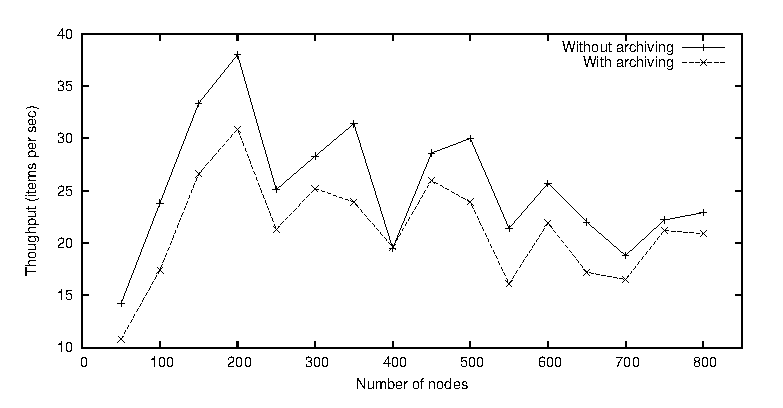
\epsfig{file=throughput.eps, width=\columnwidth}
\caption{Average throughput}
\end{center}
\end{figure}

\begin{figure}
\begin{center}
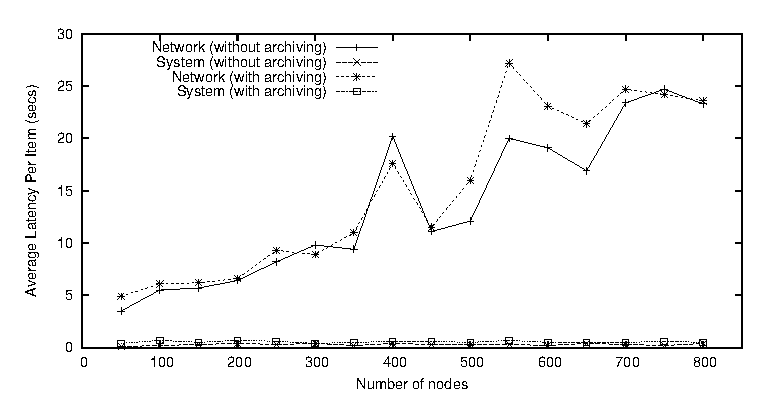
\epsfig{file=latency.eps, width=\columnwidth}
\caption{Average latencies per node}
\end{center}
\end{figure}


\begin{table*}
\begin{center}
\begin{tabular}{|l|r|r|r|r|r|r|r|r|r|r|r|r|}\hline
Num of nodes&	50&	100&	150&	200&	250&	300&	350&	400&	450&	500&	550&	600 \\ \hline\hline
Net latency per node (secs)&	9&	4&	4&	4&	8.6&	5.3&	19.1&	19.5&	14.4&	7.8&	12&	13.3 \\ \hline
Sys latency per node (secs)&	0&	0&	0&	0.3&	0.2&	0.4&	0.3&	0.1&	0.3&	0.4&	0.2&	0.7 \\ \hline
%Total Latency (secs)&	9&	4.04&	4&	4.3&	8.8&	5.8&	19.4&	19.6&	14.7&	8.2&	12.3&	14 \\ \hline
Total fetch time (secs)&	9&	5&	4&	5&	23&	9&	22&	23&	26&	14&	27&	28 \\ \hline	
Throughput (items/sec)&	5.6&	20&	37.5&	40&	10.9&	33.3&	15.9&	17.4&	17.3&	35.7&	20.4&	21.4 \\ \hline
\end{tabular}
\end{center}
\caption{Performance of Comon with no archiving}
\end{table*}


\begin{table*}
\begin{center}
\begin{tabular}{|l|r|r|r|r|r|r|r|r|r|r|r|r|}\hline
Num of nodes&	50&	100&	150&	200&	250&	300&	350&	400&	450&	500&	550&	600 \\ \hline\hline
Net latency per node (secs)&	16&	4&	4&	4&	18.9&	6&	20.6&	22&	8.4&	13&	21.8&	21.3 \\ \hline
Sys latency per node (secs)&	0.8&	1.28&	1.4&	1.8&	1.9&	1.5&	1.6&	1.3&	1.9&	1.7&	1.7&	2.2 \\ \hline
%Total Latency (secs)&	16.8&	5.28&	5.4&	5.8&	20.8&	7.5&	22.2&	23.3&	10.3&	14.7&	23.56&	23.5 \\ \hline
Total fetch time (secs)&	17&	6&	7&	7&	27&	12&	27&	30&	19&	33&	43&	43 \\ \hline
Throughput (items/sec)&	2.9&	16.7&	21.4&	28.6&	9.3&	25&	13&	13.3&	23.7&	15.2&	12.8&	14 \\ \hline
\end{tabular}
\end{center}
\caption{Performance of Comon with archiving}
\end{table*}



\bibliographystyle{jhr-alpha}
\bibliography{pads}

\appendix
\chapter{Error codes}
\label{app:error-codes}
include table listing all error codes and their meaning.
\chapter{All \PADSL{} Base Types}
\label{ap:base-types}
\cutname{base_types_appendix.html}

\section{Character Base Types}

\subsection{Fixed-width character-based encoding}

\aedBegin{}
\aedLine{char}
\aedEnd{}
\\[1ex]
The corresponding read functions are:
\begin{tinycodeaux}{\leftmargin=0in}
Perror_t Pchar_read   (P_t *pads, const Pbase_m *m, Pbase_pd *pd, Pchar *c_out);
Perror_t Pa_char_read (P_t *pads, const Pbase_m *m, Pbase_pd *pd, Pchar *c_out);
Perror_t Pe_char_read (P_t *pads, const Pbase_m *m, Pbase_pd *pd, Pchar *c_out);
\end{tinycodeaux}

\subsection{Special character counting base types}

\aedBegin{}
\aedLine{countX}
\aedLine{countXtoY}
\aedEnd{}

\begin{tinycodeaux}{\leftmargin=0in}
Perror_t PcountX     (P_t *pads, const Pbase_m *m, Puint8 x, int eor_required,
		      Pbase_pd *pd, Pint32 *res_out);
Perror_t Pa_countX   (P_t *pads, const Pbase_m *m, Puint8 x, int eor_required,
		      Pbase_pd *pd, Pint32 *res_out);
Perror_t Pe_countX   (P_t *pads, const Pbase_m *m, Puint8 x, int eor_required,
		      Pbase_pd *pd, Pint32 *res_out);

Perror_t PcountXtoY  (P_t *pads, const Pbase_m *m, Puint8 x, Puint8 y,
		      Pbase_pd *pd, Pint32 *res_out);
Perror_t Pa_countXtoY(P_t *pads, const Pbase_m *m, Puint8 x, Puint8 y,
		      Pbase_pd *pd, Pint32 *res_out);
Perror_t Pe_countXtoY(P_t *pads, const Pbase_m *m, Puint8 x, Puint8 y,
		      Pbase_pd *pd, Pint32 *res_out);
\end{tinycodeaux}

\section{String Base Types}

\subsection{Fixed-width character-based encoding}

\aedBegin{}
\aedLine{string\_FW}
\aedEnd{}

\begin{tinycodeaux}{\leftmargin=0in}
Perror_t Pstring_FW_read   (P_t *pads, const Pbase_m *m, size_t width,
			    Pbase_pd *pd, Pstring *s_out);
Perror_t Pa_string_FW_read (P_t *pads, const Pbase_m *m, size_t width,
			    Pbase_pd *pd, Pstring *s_out);
Perror_t Pe_string_FW_read (P_t *pads, const Pbase_m *m, size_t width,
			    Pbase_pd *pd, Pstring *s_out);
\end{tinycodeaux}

\subsection{Variable-width character-based encoding}

\aedBegin{}
\aedLine{string}
\aedLine{string\_ME}
\aedLine{string\_CME}
\aedLine{string\_SE}
\aedLine{string\_CSE}
\aedEnd{}

\begin{tinycodeaux}{\leftmargin=0in}
Perror_t Pstring_read      (P_t *pads, const Pbase_m *m, Pchar stopChar,
			    Pbase_pd *pd, Pstring *s_out);
Perror_t Pa_string_read    (P_t *pads, const Pbase_m *m, Pchar stopChar,
			    Pbase_pd *pd, Pstring *s_out);
Perror_t Pe_string_read    (P_t *pads, const Pbase_m *m, Pchar stopChar,
			    Pbase_pd *pd, Pstring *s_out);

Perror_t Pstring_ME_read   (P_t *pads, const Pbase_m *m, const char *matchRegexp,
			    Pbase_pd *pd, Pstring *s_out);
Perror_t Pa_string_ME_read (P_t *pads, const Pbase_m *m, const char *matchRegexp,
			    Pbase_pd *pd, Pstring *s_out);
Perror_t Pe_string_ME_read (P_t *pads, const Pbase_m *m, const char *matchRegexp,
			    Pbase_pd *pd, Pstring *s_out);

Perror_t Pstring_CME_read  (P_t *pads, const Pbase_m *m, Pregexp_t *matchRegexp,
			    Pbase_pd *pd, Pstring *s_out);
Perror_t Pa_string_CME_read(P_t *pads, const Pbase_m *m, Pregexp_t *matchRegexp,
			    Pbase_pd *pd, Pstring *s_out);
Perror_t Pe_string_CME_read(P_t *pads, const Pbase_m *m, Pregexp_t *matchRegexp,
			    Pbase_pd *pd, Pstring *s_out);

Perror_t Pstring_SE_read   (P_t *pads, const Pbase_m *m, const char *stopRegexp,
			    Pbase_pd *pd, Pstring *s_out);
Perror_t Pa_string_SE_read (P_t *pads, const Pbase_m *m, const char *stopRegexp,
			    Pbase_pd *pd, Pstring *s_out);
Perror_t Pe_string_SE_read (P_t *pads, const Pbase_m *m, const char *stopRegexp,
			    Pbase_pd *pd, Pstring *s_out);

Perror_t Pstring_CSE_read  (P_t *pads, const Pbase_m *m, Pregexp_t *stopRegexp,
			    Pbase_pd *pd, Pstring *s_out);
Perror_t Pa_string_CSE_read(P_t *pads, const Pbase_m *m, Pregexp_t *stopRegexp,
			    Pbase_pd *pd, Pstring *s_out);
Perror_t Pe_string_CSE_read(P_t *pads, const Pbase_m *m, Pregexp_t *stopRegexp,
			    Pbase_pd *pd, Pstring *s_out);
\end{tinycodeaux}

\subsection{Special string base types}

\aedBegin{}
\Pd{date}, \Pa{date}, \Pe{date}.
\aedEnd{}

\begin{tinycodeaux}{\leftmargin=0in}
Perror_t Pdate_read  (P_t *pads, const Pbase_m *m, Pchar stopChar,
		      Pbase_pd *pd, Puint32 *res_out);
Perror_t Pa_date_read(P_t *pads, const Pbase_m *m, Pchar stopChar,
		      Pbase_pd *pd, Puint32 *res_out);
Perror_t Pe_date_read(P_t *pads, const Pbase_m *m, Pchar stopChar,
		      Pbase_pd *pd, Puint32 *res_out);
\end{tinycodeaux}

\section{Integer Base Types}

\subsection{Fixed-width character-based encoding}

\aedBegin{}
\aedLine{int8\_FW}
\aedLine{int16\_FW}
\aedLine{int32\_FW}
\aedLine{int64\_FW}
\aedLine{uint8\_FW}
\aedLine{uint16\_FW}
\aedLine{uint32\_FW}
\aedLine{uint64\_FW}
\aedEnd{}

\begin{tinycodeaux}{\leftmargin=0in}
Perror_t Pa_int8_FW_read (P_t *pads, const Pbase_m *m, size_t width,
			  Pbase_pd *pd, Pint8 *res_out);
Perror_t Pa_int16_FW_read(P_t *pads, const Pbase_m *m, size_t width,
			  Pbase_pd *pd, Pint16 *res_out);
Perror_t Pa_int32_FW_read(P_t *pads, const Pbase_m *m, size_t width,
			  Pbase_pd *pd, Pint32 *res_out);
Perror_t Pa_int64_FW_read(P_t *pads, const Pbase_m *m, size_t width,
			  Pbase_pd *pd, Pint64 *res_out);

Perror_t Pa_uint8_FW_read (P_t *pads, const Pbase_m *m, size_t width,
			   Pbase_pd *pd, Puint8 *res_out);
Perror_t Pa_uint16_FW_read(P_t *pads, const Pbase_m *m, size_t width,
			   Pbase_pd *pd, Puint16 *res_out);
Perror_t Pa_uint32_FW_read(P_t *pads, const Pbase_m *m, size_t width,
			   Pbase_pd *pd, Puint32 *res_out);
Perror_t Pa_uint64_FW_read(P_t *pads, const Pbase_m *m, size_t width,
			   Pbase_pd *pd, Puint64 *res_out);

Perror_t Pe_int8_FW_read (P_t *pads, const Pbase_m *m, size_t width,
			  Pbase_pd *pd, Pint8 *res_out);
Perror_t Pe_int16_FW_read(P_t *pads, const Pbase_m *m, size_t width,
			  Pbase_pd *pd, Pint16 *res_out);
Perror_t Pe_int32_FW_read(P_t *pads, const Pbase_m *m, size_t width,
			  Pbase_pd *pd, Pint32 *res_out);
Perror_t Pe_int64_FW_read(P_t *pads, const Pbase_m *m, size_t width,
			  Pbase_pd *pd, Pint64 *res_out);

Perror_t Pe_uint8_FW_read (P_t *pads, const Pbase_m *m, size_t width,
			   Pbase_pd *pd, Puint8 *res_out);
Perror_t Pe_uint16_FW_read(P_t *pads, const Pbase_m *m, size_t width,
			   Pbase_pd *pd, Puint16 *res_out);
Perror_t Pe_uint32_FW_read(P_t *pads, const Pbase_m *m, size_t width,
			   Pbase_pd *pd, Puint32 *res_out);
Perror_t Pe_uint64_FW_read(P_t *pads, const Pbase_m *m, size_t width,
			   Pbase_pd *pd, Puint64 *res_out);

Perror_t Pint8_FW_read (P_t *pads, const Pbase_m *m, size_t width,
			Pbase_pd *pd, Pint8 *res_out);
Perror_t Pint16_FW_read(P_t *pads, const Pbase_m *m, size_t width,
			Pbase_pd *pd, Pint16 *res_out);
Perror_t Pint32_FW_read(P_t *pads, const Pbase_m *m, size_t width,
			Pbase_pd *pd, Pint32 *res_out);
Perror_t Pint64_FW_read(P_t *pads, const Pbase_m *m, size_t width,
			Pbase_pd *pd, Pint64 *res_out);

Perror_t Puint8_FW_read (P_t *pads, const Pbase_m *m, size_t width,
			 Pbase_pd *pd, Puint8 *res_out);
Perror_t Puint16_FW_read(P_t *pads, const Pbase_m *m, size_t width,
			 Pbase_pd *pd, Puint16 *res_out);
Perror_t Puint32_FW_read(P_t *pads, const Pbase_m *m, size_t width,
			 Pbase_pd *pd, Puint32 *res_out);
Perror_t Puint64_FW_read(P_t *pads, const Pbase_m *m, size_t width,
			 Pbase_pd *pd, Puint64 *res_out);
\end{tinycodeaux}

\subsection{Variable-width character-based encoding}

\aedBegin{}
\aedLine{int8}
\aedLine{int16}
\aedLine{int32}
\aedLine{int64}
\aedLine{uint8}
\aedLine{uint16}
\aedLine{uint32}
\aedLine{uint64}
\aedEnd{}

\begin{tinycodeaux}{\leftmargin=0in}
\codeallowbreaks
Perror_t Pa_int8_read (P_t *pads, const Pbase_m *m,
		       Pbase_pd *pd, Pint8 *res_out);
Perror_t Pa_int16_read(P_t *pads, const Pbase_m *m,
		       Pbase_pd *pd, Pint16 *res_out);
Perror_t Pa_int32_read(P_t *pads, const Pbase_m *m,
		       Pbase_pd *pd, Pint32 *res_out);
Perror_t Pa_int64_read(P_t *pads, const Pbase_m *m,
		       Pbase_pd *pd, Pint64 *res_out);

Perror_t Pa_uint8_read (P_t *pads, const Pbase_m *m,
			Pbase_pd *pd, Puint8 *res_out);
Perror_t Pa_uint16_read(P_t *pads, const Pbase_m *m,
			Pbase_pd *pd, Puint16 *res_out);
Perror_t Pa_uint32_read(P_t *pads, const Pbase_m *m,
			Pbase_pd *pd, Puint32 *res_out);
Perror_t Pa_uint64_read(P_t *pads, const Pbase_m *m,
			Pbase_pd *pd, Puint64 *res_out);

Perror_t Pe_int8_read (P_t *pads, const Pbase_m *m,
		       Pbase_pd *pd, Pint8 *res_out);
Perror_t Pe_int16_read(P_t *pads, const Pbase_m *m,
		       Pbase_pd *pd, Pint16 *res_out);
Perror_t Pe_int32_read(P_t *pads, const Pbase_m *m,
		       Pbase_pd *pd, Pint32 *res_out);
Perror_t Pe_int64_read(P_t *pads, const Pbase_m *m,
		       Pbase_pd *pd, Pint64 *res_out);

Perror_t Pe_uint8_read (P_t *pads, const Pbase_m *m,
			Pbase_pd *pd, Puint8 *res_out);
Perror_t Pe_uint16_read(P_t *pads, const Pbase_m *m,
			Pbase_pd *pd, Puint16 *res_out);
Perror_t Pe_uint32_read(P_t *pads, const Pbase_m *m,
			Pbase_pd *pd, Puint32 *res_out);
Perror_t Pe_uint64_read(P_t *pads, const Pbase_m *m,
			Pbase_pd *pd, Puint64 *res_out);

Perror_t Pint8_read (P_t *pads, const Pbase_m *m,
		     Pbase_pd *pd, Pint8 *res_out);
Perror_t Pint16_read(P_t *pads, const Pbase_m *m,
		     Pbase_pd *pd, Pint16 *res_out);
Perror_t Pint32_read(P_t *pads, const Pbase_m *m,
		     Pbase_pd *pd, Pint32 *res_out);
Perror_t Pint64_read(P_t *pads, const Pbase_m *m,
		     Pbase_pd *pd, Pint64 *res_out);

Perror_t Puint8_read (P_t *pads, const Pbase_m *m,
		      Pbase_pd *pd, Puint8 *res_out);
Perror_t Puint16_read(P_t *pads, const Pbase_m *m,
		      Pbase_pd *pd, Puint16 *res_out);
Perror_t Puint32_read(P_t *pads, const Pbase_m *m,
		      Pbase_pd *pd, Puint32 *res_out);
Perror_t Puint64_read(P_t *pads, const Pbase_m *m,
		      Pbase_pd *pd, Puint64 *res_out);
\end{tinycodeaux}

\subsection{Raw binary encoding}

\bBegin{}
\bLine{int8}
\bLine{int16}
\bLine{int32}
\bLine{int64}
\bLine{uint8}
\bLine{uint16}
\bLine{uint32}
\bLine{uint64}
\bEnd{}

\begin{tinycodeaux}{\leftmargin=0in}
\codeallowbreaks
Perror_t Pb_int8_read (P_t *pads, const Pbase_m *m,
		       Pbase_pd *pd, Pint8 *res_out);
Perror_t Pb_int16_read(P_t *pads, const Pbase_m *m,
		       Pbase_pd *pd, Pint16 *res_out);
Perror_t Pb_int32_read(P_t *pads, const Pbase_m *m,
		       Pbase_pd *pd, Pint32 *res_out);
Perror_t Pb_int64_read(P_t *pads, const Pbase_m *m,
		       Pbase_pd *pd, Pint64 *res_out);

Perror_t Pb_uint8_read (P_t *pads, const Pbase_m *m,
			Pbase_pd *pd, Puint8 *res_out);
Perror_t Pb_uint16_read(P_t *pads, const Pbase_m *m,
			Pbase_pd *pd, Puint16 *res_out);
Perror_t Pb_uint32_read(P_t *pads, const Pbase_m *m,
			Pbase_pd *pd, Puint32 *res_out);
Perror_t Pb_uint64_read(P_t *pads, const Pbase_m *m,
			Pbase_pd *pd, Puint64 *res_out);
\end{tinycodeaux}

\subsection{Serialize binary encoding}

\sbBegin{}
\sbLine{int8}
\sbLine{int16}
\sbLine{int32}
\sbLine{int64}
\sbLine{uint8}
\sbLine{uint16}
\sbLine{uint32}
\sbLine{uint64}
\bEnd{}

\begin{tinycodeaux}{\leftmargin=0in}
\codeallowbreaks
Perror_t Psbl_int8_read    (P_t *pads, const Pbase_m *m, Puint32 num_bytes,
			    Pbase_pd *pd, Pint8 *res_out);
Perror_t Psbl_int16_read   (P_t *pads, const Pbase_m *m, Puint32 num_bytes,
			    Pbase_pd *pd, Pint16 *res_out);
Perror_t Psbl_int32_read   (P_t *pads, const Pbase_m *m, Puint32 num_bytes,
			    Pbase_pd *pd, Pint32 *res_out);
Perror_t Psbl_int64_read   (P_t *pads, const Pbase_m *m, Puint32 num_bytes,
			    Pbase_pd *pd, Pint64 *res_out);

Perror_t Psbl_uint8_read   (P_t *pads, const Pbase_m *m, Puint32 num_bytes,
			    Pbase_pd *pd, Puint8 *res_out);
Perror_t Psbl_uint16_read  (P_t *pads, const Pbase_m *m, Puint32 num_bytes,
			    Pbase_pd *pd, Puint16 *res_out);
Perror_t Psbl_uint32_read  (P_t *pads, const Pbase_m *m, Puint32 num_bytes,
			    Pbase_pd *pd, Puint32 *res_out);
Perror_t Psbl_uint64_read  (P_t *pads, const Pbase_m *m, Puint32 num_bytes,
			    Pbase_pd *pd, Puint64 *res_out);

Perror_t Psbh_int8_read    (P_t *pads, const Pbase_m *m, Puint32 num_bytes,
			    Pbase_pd *pd, Pint8 *res_out);
Perror_t Psbh_int16_read   (P_t *pads, const Pbase_m *m, Puint32 num_bytes,
			    Pbase_pd *pd, Pint16 *res_out);
Perror_t Psbh_int32_read   (P_t *pads, const Pbase_m *m, Puint32 num_bytes,
			    Pbase_pd *pd, Pint32 *res_out);
Perror_t Psbh_int64_read   (P_t *pads, const Pbase_m *m, Puint32 num_bytes,
			    Pbase_pd *pd, Pint64 *res_out);

Perror_t Psbh_uint8_read   (P_t *pads, const Pbase_m *m, Puint32 num_bytes,
			    Pbase_pd *pd, Puint8 *res_out);
Perror_t Psbh_uint16_read  (P_t *pads, const Pbase_m *m, Puint32 num_bytes,
			    Pbase_pd *pd, Puint16 *res_out);
Perror_t Psbh_uint32_read  (P_t *pads, const Pbase_m *m, Puint32 num_bytes,
			    Pbase_pd *pd, Puint32 *res_out);
Perror_t Psbh_uint64_read  (P_t *pads, const Pbase_m *m, Puint32 num_bytes,
			    Pbase_pd *pd, Puint64 *res_out);
\end{tinycodeaux}

\subsection{EBC and BCD encoding}

\cBegin{}
\cLine{int8}
\cLine{int16}
\cLine{int32}
\cLine{int64}
\cLine{uint8}
\cLine{uint16}
\cLine{uint32}
\cLine{uint64}
\cEnd{}

\begin{tinycodeaux}{\leftmargin=0in}
\codeallowbreaks
Perror_t Pebc_int8_read   (P_t *pads, const Pbase_m *m, Puint32 num_digits,
			   Pbase_pd *pd, Pint8 *res_out);
Perror_t Pebc_int16_read  (P_t *pads, const Pbase_m *m, Puint32 num_digits,
			   Pbase_pd *pd, Pint16 *res_out);
Perror_t Pebc_int32_read  (P_t *pads, const Pbase_m *m, Puint32 num_digits,
			   Pbase_pd *pd, Pint32 *res_out);
Perror_t Pebc_int64_read  (P_t *pads, const Pbase_m *m, Puint32 num_digits,
			   Pbase_pd *pd, Pint64 *res_out);

Perror_t Pebc_uint8_read  (P_t *pads, const Pbase_m *m, Puint32 num_digits,
			   Pbase_pd *pd, Puint8 *res_out);
Perror_t Pebc_uint16_read (P_t *pads, const Pbase_m *m, Puint32 num_digits,
			   Pbase_pd *pd, Puint16 *res_out);
Perror_t Pebc_uint32_read (P_t *pads, const Pbase_m *m, Puint32 num_digits,
			   Pbase_pd *pd, Puint32 *res_out);
Perror_t Pebc_uint64_read (P_t *pads, const Pbase_m *m, Puint32 num_digits,
			   Pbase_pd *pd, Puint64 *res_out);

Perror_t Pbcd_int8_read   (P_t *pads, const Pbase_m *m, Puint32 num_digits,
			   Pbase_pd *pd, Pint8 *res_out);
Perror_t Pbcd_int16_read  (P_t *pads, const Pbase_m *m, Puint32 num_digits,
			   Pbase_pd *pd, Pint16 *res_out);
Perror_t Pbcd_int32_read  (P_t *pads, const Pbase_m *m, Puint32 num_digits,
			   Pbase_pd *pd, Pint32 *res_out);
Perror_t Pbcd_int64_read  (P_t *pads, const Pbase_m *m, Puint32 num_digits,
			   Pbase_pd *pd, Pint64 *res_out);

Perror_t Pbcd_uint8_read  (P_t *pads, const Pbase_m *m, Puint32 num_digits,
			   Pbase_pd *pd, Puint8 *res_out);
Perror_t Pbcd_uint16_read (P_t *pads, const Pbase_m *m, Puint32 num_digits,
			   Pbase_pd *pd, Puint16 *res_out);
Perror_t Pbcd_uint32_read (P_t *pads, const Pbase_m *m, Puint32 num_digits,
			   Pbase_pd *pd, Puint32 *res_out);
Perror_t Pbcd_uint64_read (P_t *pads, const Pbase_m *m, Puint32 num_digits,
			   Pbase_pd *pd, Puint64 *res_out);
\end{tinycodeaux}

\section{Floating Point Base Types}

\subsection{Fixed-width character-based encoding}

\aedBegin{}
\aedLine{float32\_FW}
\aedLine{float64\_FW}
\aedEnd{}

\begin{tinycodeaux}{\leftmargin=0in}
\end{tinycodeaux}

\subsection{Variable-width character-based encoding}

\aedBegin{}
\aedLine{float32}
\aedLine{float64}
\aedEnd{}

\begin{tinycodeaux}{\leftmargin=0in}
\end{tinycodeaux}

\subsection{Raw binary encoding}

\bBegin{}
\bLine{float32}
\bLine{float64}
\bEnd{}

\begin{tinycodeaux}{\leftmargin=0in}
\end{tinycodeaux}

\subsection{Serialized binary encoding}

\sbBegin{}
\sbLine{float32}
\sbLine{float64}
\sbEnd{}

\begin{tinycodeaux}{\leftmargin=0in}
\end{tinycodeaux}

\section{Fixed Point Base Types}

\subsection{Serialized binary encoding}

\sbBegin{}
\sbLine{fpoint8}
\sbLine{fpoint16}
\sbLine{fpoint32}
\sbLine{fpoint64}
\sbLine{ufpoint8}
\sbLine{ufpoint16}
\sbLine{ufpoint32}
\sbLine{ufpoint64}
\bEnd{}

\begin{tinycodeaux}{\leftmargin=0in}
\codeallowbreaks
Perror_t Psbl_fpoint8_read    (P_t *pads, const Pbase_m *m, Puint32 num_bytes, Puint32 d_exp,
			       Pbase_pd *pd, Pfpoint8 *res_out);
Perror_t Psbl_fpoint16_read   (P_t *pads, const Pbase_m *m, Puint32 num_bytes, Puint32 d_exp,
			       Pbase_pd *pd, Pfpoint16 *res_out);
Perror_t Psbl_fpoint32_read   (P_t *pads, const Pbase_m *m, Puint32 num_bytes, Puint32 d_exp,
			       Pbase_pd *pd, Pfpoint32 *res_out);
Perror_t Psbl_fpoint64_read   (P_t *pads, const Pbase_m *m, Puint32 num_bytes, Puint32 d_exp,
			       Pbase_pd *pd, Pfpoint64 *res_out);

Perror_t Psbl_ufpoint8_read   (P_t *pads, const Pbase_m *m, Puint32 num_bytes, Puint32 d_exp,
			       Pbase_pd *pd, Pufpoint8 *res_out);
Perror_t Psbl_ufpoint16_read  (P_t *pads, const Pbase_m *m, Puint32 num_bytes, Puint32 d_exp,
			       Pbase_pd *pd, Pufpoint16 *res_out);
Perror_t Psbl_ufpoint32_read  (P_t *pads, const Pbase_m *m, Puint32 num_bytes, Puint32 d_exp,
			       Pbase_pd *pd, Pufpoint32 *res_out);
Perror_t Psbl_ufpoint64_read  (P_t *pads, const Pbase_m *m, Puint32 num_bytes, Puint32 d_exp,
			       Pbase_pd *pd, Pufpoint64 *res_out);

Perror_t Psbh_fpoint8_read    (P_t *pads, const Pbase_m *m, Puint32 num_bytes, Puint32 d_exp,
			       Pbase_pd *pd, Pfpoint8 *res_out);
Perror_t Psbh_fpoint16_read   (P_t *pads, const Pbase_m *m, Puint32 num_bytes, Puint32 d_exp,
			       Pbase_pd *pd, Pfpoint16 *res_out);
Perror_t Psbh_fpoint32_read   (P_t *pads, const Pbase_m *m, Puint32 num_bytes, Puint32 d_exp,
			       Pbase_pd *pd, Pfpoint32 *res_out);
Perror_t Psbh_fpoint64_read   (P_t *pads, const Pbase_m *m, Puint32 num_bytes, Puint32 d_exp,
			       Pbase_pd *pd, Pfpoint64 *res_out);

Perror_t Psbh_ufpoint8_read   (P_t *pads, const Pbase_m *m, Puint32 num_bytes, Puint32 d_exp,
			       Pbase_pd *pd, Pufpoint8 *res_out);
Perror_t Psbh_ufpoint16_read  (P_t *pads, const Pbase_m *m, Puint32 num_bytes, Puint32 d_exp,
			       Pbase_pd *pd, Pufpoint16 *res_out);
Perror_t Psbh_ufpoint32_read  (P_t *pads, const Pbase_m *m, Puint32 num_bytes, Puint32 d_exp,
			       Pbase_pd *pd, Pufpoint32 *res_out);
Perror_t Psbh_ufpoint64_read  (P_t *pads, const Pbase_m *m, Puint32 num_bytes, Puint32 d_exp,
			       Pbase_pd *pd, Pufpoint64 *res_out);
\end{tinycodeaux}

\subsection{EBC and BCD encoding}

\cBegin{}
\cLine{fpoint8}
\cLine{fpoint16}
\cLine{fpoint32}
\cLine{fpoint64}
\cLine{ufpoint8}
\cLine{ufpoint16}
\cLine{ufpoint32}
\cLine{ufpoint64}
\cEnd{}

\begin{tinycodeaux}{\leftmargin=0in}
\codeallowbreaks
Perror_t Pebc_fpoint8_read   (P_t *pads, const Pbase_m *m, Puint32 num_digits, Puint32 d_exp,
			      Pbase_pd *pd, Pfpoint8 *res_out);
Perror_t Pebc_fpoint16_read  (P_t *pads, const Pbase_m *m, Puint32 num_digits, Puint32 d_exp,
			      Pbase_pd *pd, Pfpoint16 *res_out);
Perror_t Pebc_fpoint32_read  (P_t *pads, const Pbase_m *m, Puint32 num_digits, Puint32 d_exp,
			      Pbase_pd *pd, Pfpoint32 *res_out);
Perror_t Pebc_fpoint64_read  (P_t *pads, const Pbase_m *m, Puint32 num_digits, Puint32 d_exp,
			      Pbase_pd *pd, Pfpoint64 *res_out);

Perror_t Pebc_ufpoint8_read  (P_t *pads, const Pbase_m *m, Puint32 num_digits, Puint32 d_exp,
			      Pbase_pd *pd, Pufpoint8 *res_out);
Perror_t Pebc_ufpoint16_read (P_t *pads, const Pbase_m *m, Puint32 num_digits, Puint32 d_exp,
			      Pbase_pd *pd, Pufpoint16 *res_out);
Perror_t Pebc_ufpoint32_read (P_t *pads, const Pbase_m *m, Puint32 num_digits, Puint32 d_exp,
			      Pbase_pd *pd, Pufpoint32 *res_out);
Perror_t Pebc_ufpoint64_read (P_t *pads, const Pbase_m *m, Puint32 num_digits, Puint32 d_exp,
			      Pbase_pd *pd, Pufpoint64 *res_out);

Perror_t Pbcd_fpoint8_read   (P_t *pads, const Pbase_m *m, Puint32 num_digits, Puint32 d_exp,
			      Pbase_pd *pd, Pfpoint8 *res_out);
Perror_t Pbcd_fpoint16_read  (P_t *pads, const Pbase_m *m, Puint32 num_digits, Puint32 d_exp,
			      Pbase_pd *pd, Pfpoint16 *res_out);
Perror_t Pbcd_fpoint32_read  (P_t *pads, const Pbase_m *m, Puint32 num_digits, Puint32 d_exp,
			      Pbase_pd *pd, Pfpoint32 *res_out);
Perror_t Pbcd_fpoint64_read  (P_t *pads, const Pbase_m *m, Puint32 num_digits, Puint32 d_exp,
			      Pbase_pd *pd, Pfpoint64 *res_out);

Perror_t Pbcd_ufpoint8_read  (P_t *pads, const Pbase_m *m, Puint32 num_digits, Puint32 d_exp,
			      Pbase_pd *pd, Pufpoint8 *res_out);
Perror_t Pbcd_ufpoint16_read (P_t *pads, const Pbase_m *m, Puint32 num_digits, Puint32 d_exp,
			      Pbase_pd *pd, Pufpoint16 *res_out);
Perror_t Pbcd_ufpoint32_read (P_t *pads, const Pbase_m *m, Puint32 num_digits, Puint32 d_exp,
			      Pbase_pd *pd, Pufpoint32 *res_out);
Perror_t Pbcd_ufpoint64_read (P_t *pads, const Pbase_m *m, Puint32 num_digits, Puint32 d_exp,
			      Pbase_pd *pd, Pufpoint64 *res_out);

\end{tinycodeaux}

\end{document}
